%!TEX encoding = UTF-8 Unicode
% ================================================================================
\documentclass[
    fontsize=12pt,
    headings=small,
    parskip=half,           % Ersetzt manuelles Setzen von parskip/parindent.
    bibliography=totoc,
    numbers=noenddot,       % Entfernt den letzten Punkt der Kapitelnummern.
    open=any,               % Kapitel kann auf jeder Seite beginnen.
%   final                   % Entfernt alle todonotes und den Entwurfstempel.
    ]{scrreprt}
% ===================================Praeambel==================================
%!TEX encoding = UTF-8 Unicode
%!TEX root = hinweiseabschlussarbeit.tex

% Kodierung, Sprache, Patches {{{
\usepackage[T1]{fontenc}    % Ausgabekodierung; ermöglicht Akzente und Umlaute
                            %  sowie korrekte Silbentrennung.
\usepackage[utf8]{inputenc} % Erlaubt die direkte Eingabe spezieller Zeichen;
                            %  utf8 muss die Eingabekodierung des Editors sein.
\usepackage[ngerman]{babel} % Deutsche Sprachanpassungen (z.B. Überschriften).
\usepackage{microtype}      % Optimale Randausrichtung und Skalierung.
\usepackage[
    autostyle,
    ]{csquotes}             % Korrekte Anführungszeichen in der Literaturliste.
%\usepackage{fixltx2e}      % Patches fuer LaTeX2e - seit 2015 nicht mehr nötig
\usepackage{scrhack}        % Verhindert Warnungen mit älteren Paketen.
\usepackage[
  newcommands
]{ragged2e}                 % Verbesserte \ragged...Befehle
\PassOptionsToPackage{
  hyphens
}{url}                      % Sorgt für URL-Umbrüche in Fußzeilen u. Literatur
% }}}

% Schriftarten {{{
\usepackage{mathptmx}       % Times; modifies the default serif and math fonts
\usepackage[scaled=.92]{helvet}% modifies the sans serif font
\usepackage{courier}        % modifies the monospace font
% }}}

% Biblatex {{{
\usepackage[
    style=alphabetic,
    backend=biber,
    %backref=true
    ]{biblatex}             % Biblatex mit alphabetischem Style und biber.
\bibliography{literaturliste.bib} % Dateiname der bib-Datei.
\DeclareFieldFormat*{title}{
    \mkbibemph{#1}}         % Make titles italics
% }}}

% Dokument- und Texteinstellungen {{{
\usepackage[
    a4paper,
    margin=2.54cm,
    marginparwidth=2.0cm,
    footskip=1.0cm
    ]{geometry}             % Ersetzt 'a4wide'.
\clubpenalty=10000          % Keine Einzelzeile am Beginn eines Absatzes
                            %  (Schusterjungen).
\widowpenalty=10000         % Keine Einzelzeile am Ende eines Absatzes
\displaywidowpenalty=10000  %  (Hurenkinder).
\usepackage{floatrow}       % Zentriert alle Floats
\usepackage{ifdraft}        % Ermöglicht \ifoptionfinal{true}{false}
\pagestyle{plain}           % keine Kopfzeilen
% \sloppy                    % großzügige Formatierungsweise
\deffootnote{1em}{1em}{
  \thefootnotemark.\ }      % Verbessert Layout mehrzeiliger Fußnoten
\ifdefined\chapterformat
	\renewcommand*{\chapterformat}{% Hübscht Kapitelüberschrift mit senkrechtem 
		\thechapter\enskip%          grauen Balken zwischen Nummer und Text auf
		\textcolor{gray!50}{\rule[-\dp\strutbox]{2pt}{\baselineskip}}\enskip
	}
\fi
%\setkomafont{disposition}{\normalcolor\bfseries} % Aus der KOMA-Skript-Anleitung: „Mit dieser Änderung verzichten Sie darauf, für alle Gliederungsebenen serifenlose Schrift voreinzustellen“

\makeatletter
\AtBeginDocument{%
    \hypersetup{%
        pdftitle = {\@title},
        pdfauthor  = \@author,
    }
}
\makeatother
% }}}

\newcommand*\rot[1]{\rotatebox{90}{#1}}

% Weitere Pakete {{{
\usepackage{graphicx}       % Einfügen von Graphiken.
\usepackage{tabu}           % Einfügen von Tabellen.
\usepackage{multirow}       % Tabellenzeilen zusammenfassen.
\usepackage{multicol}       % Tabellenspalten zusammenfassen.
\usepackage{booktabs}       % Schönere Tabellen (\toprule\midrule\bottomrule).
\usepackage[nocut]{thmbox}  % Theorembox bspw. für Angreifermodell.
\usepackage{amsmath}        % Erweiterte Handhabung mathematischer Formeln.
\usepackage{amssymb}        % Erweiterte mathematische Symbole.
\usepackage{rotating}
\usepackage{longtable}      % for 'longtable' environment
\usepackage{pdflscape}      % for 'landscape' environment
\usepackage{xltabular}
\usepackage[
    printonlyused
    ]{acronym}              % Abkürzungsverzeichnis
\usepackage[
    colorinlistoftodos,
    textsize=tiny,          % Notizen und TODOs - mit der todonotes.sty von
    \ifoptionfinal{disable}{}%  Benjamin Kellermann ist das Package "changebar"
    ]{todonotes}            %  bereits integriert.
\usepackage[
    breaklinks,
    hidelinks,
    pdfdisplaydoctitle,
    pdfpagemode = {UseOutlines},
    pdfpagelabels,
    ]{hyperref}             % Sprungmarken im PDF. Lädt das URL-Paket.
    \urlstyle{rm}           % Entfernt die Formattierung von URLs.
%\usepackage{breakurl}
%\def\UrlBreaks{\do\/\do-}
\usepackage{listings}       % Spezielle Umgebung für Quelltextformatierung.
    \lstset{                
        language=C,
        breaklines=true,
        breakatwhitespace=true,
        frame=l,            % Linie links: l, doppelt: L
		framerule=2.5pt,    % Dicke der Linie
		rulecolor=\color{gray},% Farbe der Linie
        captionpos=b,
        xleftmargin=6ex,
        tabsize=4,
        numbers=left,
        numberstyle=\ttfamily\footnotesize,
        basicstyle=\ttfamily\footnotesize,
        keywordstyle=\bfseries\color{green!50!black},
        commentstyle=\itshape\color{magenta!90!black},
        identifierstyle=\ttfamily,
        stringstyle=\color{orange!90!black},
        showstringspaces=false,
        }

\usepackage{algorithm}
\usepackage{algpseudocode}
%\usepackage{filecontents}  % Direktes Einfügen von Dateiinhalt. Wird hier für
                            %  die Verwendung einer .bib-Datei in dieser .tex-
                            %  Datei benötigt.
% }}}

% ===================================Dokument===================================

\title{Intrusion detection for OAuth}
\author{Florian Nehmer}
\date{06.01.2023} % Falls ein bestimmtes Datum eingesetzt werden soll, einfach
                    %  diese Zeile aktivieren.

\begin{document}

\begin{titlepage}% {{{
	
\includegraphics[width=6.8cm]{./pic/up-uhh-logo-u-2010-u-farbe-u-rgb.pdf}
	\begin{center}\Large
		\vfill
		Masterarbeit
		\vfill
		\makeatletter
		{\Large\textsf{\textbf{\@title}}\par}
		\makeatother
		\vfill
		vorgelegt von
		\par\bigskip
		\makeatletter
		{\@author} \par
		\makeatother
		Matrikelnummer 6417446 \par
		Studiengang Informatik
		\vfill
		MIN-Fakultät \par
		Fachbereich Informatik
		\vfill
		\makeatletter
		eingereicht am {\@date}
		\makeatother
		\vfill
		Betreuer: Pascal Wichmann, M.\,Sc. Informatik \par
		Erstgutachter: Prof. Dr.-Ing. Hannes Federrath \par
		Zweitgutachter: Pascal Wichmann, M.\,Sc. Informatik.
	\end{center}
	\ifoptionfinal{}{
	\begin{tikzpicture}[remember picture, overlay]
		\node[draw, red, font=\ttfamily\bfseries\Large, xshift=30mm, yshift=238mm,
			rotate=340, text centered, text width=6cm, very thick, rounded
			corners=4mm] at (current page.south) {Entwurf vom \today};
	\end{tikzpicture}
	% ====> Delete me
	\begin{tikzpicture}[overlay]
		\node[draw, blue, font=\sffamily\Large, xshift=0mm, yshift=210mm, rotate=0, text centered, rounded corners=1mm] at (current page.south) {Muster des Deckblatts für Abschlussarbeiten};
	\end{tikzpicture}
	% <==== /Delete me
	}
\end{titlepage}% }}}

\chapter*{Aufgabenstellung}
OAuth [RFC6749] is a widely used authentication protocol, which is typically used between multiple actors, such as different organizations. As authentication is at the core of application security, it is specifically essential to prevent attacks on the authentication.

The tasks of this thesis are as follows: Firstly, a systematic literature study should be performed on existing properties and attacks on the OAuth protocol or its implementations. Secondly, the thesis should design protection strategies for the threats that are not sufficiently solved in existing solutions. Two options for this step are (i) the utilization of anomaly-based intrusion detection for OAuth and (ii) specification-based intrusion detection for OAuth. Thirdly, the thesis should evaluate the security of the designed architecture and compare it to other solutions.

\chapter*{Zusammenfassung}

Für die eilige Leserin bzw. den eiligen Leser sollen auf etwa einer halben, maximal einer Seite die wichtigsten Inhalte, Erkenntnisse, Neuerungen bzw. Ergebnisse der Arbeit beschrieben werden.

Durch eine solche Zusammenfassung (im Engl. auch Abstract genannt) am Anfang der Arbeit wird die Arbeit deutlich aufgewertet. Hier sollte vermittelt werden, warum man die Arbeit lesen sollte.

\tableofcontents

\chapter{Introduction}
\label{chap:introduction}
In the evolving landscape of internet services, the OAuth (Open Authorization) framework is an ever-growing popular tool that allows users to integrate their existing accounts holding personal data seamlessly into different online services. As OAuth offers diverse possibilities for various use cases to handle authorization, the standard has grown in complexity over time. There are formal analyses of the security of OAuth, which aim to prove the security of the standard itself \cite{fett2016comprehensive}, but with this large complexity comes great responsibility when implementing the protocol. A study by Philippaerts et al. conducted in 2022 shows that 97 of 100 popular OAuth providers leave at least one known OAuth threat unmitigated, with an average of four unmitigated threats per provider \cite{philippaerts2022oauch}. This study shows that many OAuth implementations are still flawed, and it did not even include the realization of millions of OAuth clients, which potentially could also have flawed implementations. Adding to that picture of the current OAuth threat landscape, the introduction of new browser features, as demonstrated by the number one of the top ten web hacking techniques of 2022 published by the company PortSwigger \cite{kettle2022}, revealed even newer and more niche attack vectors on OAuth as well. This concerning situation in the threat landscape of OAuth is not hopeless in any way, more than that, this condition should be the reason that it gets addressed appropriately. One way to achieve more trust in operating OAuth services is to detect intrusion attempts through OAuth flaws as early as possible to allow OAuth providers to react adequately and reduce damages. This can be achieved by utilizing anomaly detection techniques, even identifying unknown attack vectors, which is especially useful in an ever-changing threat landscape.


\section{Research Goals}
This research includes two primary goals. The first goal is to provide an overview of the current threat landscape of the OAuth 2.0 protocol, including potential countermeasures by suggesting a classification. 

Based on the knowledge gained by evaluating the threat landscape, the second goal is to test the effectiveness of common anomaly-based intrusion detection techniques on the application layer data of the protocol. To achieve this goal, two clustering algorithms using the protocol data encoded into word embeddings are implemented and compared to each other by their effectiveness.


\section{Outline}
While this chapter served to introduce the issues with the current threat landscape of OAuth and the motivation and approach to address them, the subsequent chapters are structured as follows:

Chapter \ref{chap:fundamental_knowledge} provides fundamental knowledge about the OAuth authorization framework, including its different modes of operation and its future outlook. It also introduces the theory of intrusion detection systems based on recent taxonomies. The chapter ends by describing the different algorithms utilized to implement the anomaly-based intrusion detection approach applied in this work. 

Chapter \ref{chap:related_work} presents related research in the realm of OAuth security in general and intrusion detection approaches utilizing Word2Vec embeddings and clustering algorithms as this work applies them.

Chapter \ref{chap:oauth_security} continues by laying out the different threats the implementation of OAuth bears and presents the current state of countermeasures to be applied. The chapter finishes with a suggestion for a classification of the various threats in the context of their countermeasures.

Chapter \ref{chap:experimental_analysis} starts by giving a detailed description of the implementation of the experiments, including the OAuth environment, the dataset generation, and the algorithmic intrusion detection method. It continues by presenting and comparing the effectiveness of the different methods as the results of the experiments.

Chapter \ref{chap:conclusion} ends this work with a résumé of this work and an outlook for future work.


\chapter{Fundamental Knowledge}
\label{chap:fundamental_knowledge}
The OAuth authorization framework is complex and extensive as it has been refined and extended through several standards over the last 11 years. Securing applications using the OAuth protocol, therefore, leads to various considerations. Consequently, section 1 introduces the essential aspects and vocabulary of the OAuth authorization framework in the web context to form an understanding of the security-relevant parts of the protocol.

As one of the main goals of this thesis is to experiment with techniques to detect attacks on services using OAuth, section 2 provides an exploration of intrusion detection systems and the different ways to categorize them.

In the last part of this chapter, section 3 concludes with a description and depiction of the different algorithms used in the experiments.

\section{OAuth 2.0 protocol}
The Open Authorization 2.0 protocol nowadays often referred to as the
\emph{OAuth} protocol, is an authorization framework, that allows third-party
applications to gain limited access to resources in a different location on
behalf of the party, that owns these resources. For many users of the Internet,
it is in practice the protocol behind the ``\emph{Sign in with ...}'' button.
The current standard, first defined in 2012 in RFC6749, is already the
successor of the OAuth 1.0 standard, which was officially published in 2010 by
the IETF in RFC5849 \cite{hammer2010rfc}. In the meantime, several extensions
for the protocol were published as standards and technical reports. These
extensions include new functionalities for the protocol e.g. the ability to use
the protocol with devices like smart TVs and printers \cite{denniss2019oauth}
or documents, which describe several security considerations when implementing
the protocol in practice \cite{lodderstedt2020oauth}. As a whole, the OAuth
working group of the Internet Engineering Task Force (IETF) submitted a total
of 30 Request for Comments (RFCs) and 16 active drafts, from which 7 are active
individual drafts. Table X shows a complete list of all OAuth 2.0. related IETF
submissions by the OAuth working group. 

\subsection{Involved parties}
Because the OAuth protocol is very diverse and complex, as it is a
whole authorization framework it makes sense to narrow it down to its core
features. Starting with the involved parties in the protocol. In general there
are four parties involved in the most common OAuth protocol modes:

\begin{itemize} 

    \item Resource owner: The resource owner is the entity that owns or is
        allowed to manage protected resources. The resource owner might grant
        access to these resources. 

    \item Resource server: The resource server is the server, where the
        protected resources are stored. It can accept or decline authorization
        tokens, which it receives from the client. 

    \item Client: The client is an entity, which makes requests to get access
        to the protected resources, on behalf of the resource owner. 
        
    \item Authorization server: The server, that manages access to the
        protected data. It issues access tokens to the client after successful
        authentication of the resource owner. 

\end{itemize}

Depending on the protocol mode, these four parties or in some cases three
parties exchange different messages in variable ways. In general, there are two
different types of messages, which are explained in the next section.

\subsection{Front-channel and Back-channel messages}

Regarding security considerations messages of the OAuth framework can be
categorized into two main categories, \emph{front-channel} and
\emph{back-channel}. As the protocol is mostly used in the application layer
using HTTP and TLS, \emph{front-channel} means that the message is transported
via the \emph{Request-URI} \cite[Sec. 5.1.2]{fielding1999hypertext} e.g. by
using query parameters. \emph{Back-channel} means on the other hand that the
message is transported via the HTTP message body. In other words, back-channel
messages are transported in one TCP connection, between caller and receiver,
whereas front-channel messages use redirects. \cite[p. 338]{belfaik2022single}.

\subsection{Grant Types}
The protocol flow is dependent on the protocol mode. In the case of OAuth the
different protocol modes are called \emph{Grant types}, as the modes differ on
how the authorization is granted to the resource owner via the client.

\subsubsection{Authorization Code Grant}
According to a recent study, the authorization code grant mode of OAuth is the
most used protocol mode for OAuth on the internet
\cite[Table1]{philippaerts2022oauch}. It is offered by more than 90\% of common 
identity providers.

In this mode illustrated in Figure 2.1, a resource owner aiming to access
protected data via a REST API utilizes a user agent, in this case the web
browser, to interact with a client application that executes API requests
through the user agent. The process begins as the client redirects the user
agent to the authorization server through the front channel. The message
contains a client ID, a redirect URL and a state. The client ID is a unique
identifier of the protected resource. The redirect URI is the location the user
agent is redirected to after authentication. The state can hold any string
value and is most commonly used for CSRF tokens. The authorization server now
asks the resource owner for authentication. If the resource owner is
authenticated and is allowed to access the desired protected resources, the
user agent gets redirected back using the redirect URI. This means that the
message is again sent via the front channel and contains now an authorization
code and the state. Using the valid authorization code and the state, the
client proceeds to request an access token via the back channel at the
authorization server. With the acquired access token the client follows with
the request of the desired protected resource at the resource server.

\begin{figure}[ht]
	\sffamily\footnotesize
	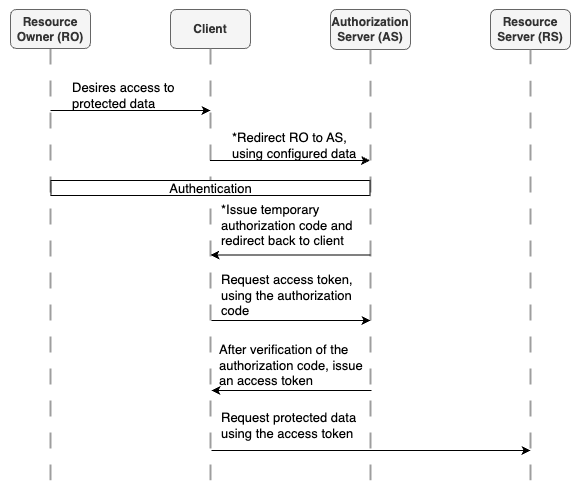
\includegraphics[width=0.75\textwidth]{pic/authorization_code_grant.png}
	\unitlength=0.75mm
	\special{em:linewidth 0.4pt}
	\linethickness{0.4pt}
	\caption{Authorization Code Grant without any extensions}
	\label{fig:auth_code_grant}
\end{figure}

\subsubsection{Implicit Grant}
The Implicit Grant was introduced at a time when there were no mechanisms like Cross-Origin resource sharing implemented in browsers, to share content from different domains. It is a predecessor of the authorization code flow and works similarly with the difference of leaving out the exchanging of the
authorization code step as visualized in figure \ref{fig:implicit_grant}. Instead, the access token is sent via the front
channel directly from the authorization server to the client. This leaves open more attack vectors for example by utilizing the browser history or by
simplifying access token injection \cite{lodderstedt2020oauth}. The Implicit
Grant is officially deprecated, but still has its relevance, as it is still
offered by 37\% of common identity providers \cite{philippaerts2022oauch}.

\begin{figure}[ht]
	\sffamily\footnotesize
	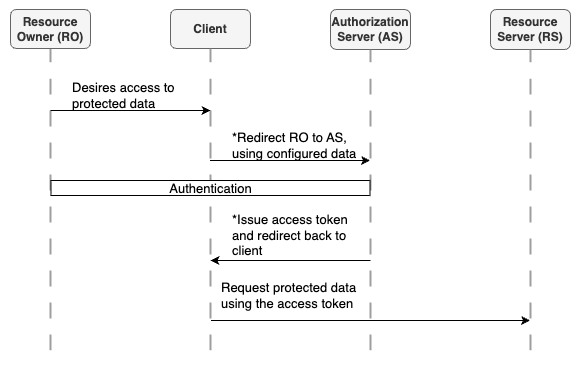
\includegraphics[width=0.75\textwidth]{pic/implicit_grant.png}
	\unitlength=0.75mm
	\special{em:linewidth 0.4pt}
	\linethickness{0.4pt}
	\caption{Implicit Grant}
	\label{fig:implicit_grant}
\end{figure}

\subsubsection{Resource Owner Password Credentials Grant}
This grant type is special in the way that the client is providing its
authentication credentials for the authorization provider to the resource
provider instead, as illustrated in figure \ref{fig:resource_owner_password_credentials_grant}. The resource provider than uses the credentials to retrieve
authorization from the authorization provider. This grant type is only feasible
for the scenario, that the resource provider is trusted completely \cite[Sec.
4.3.]{hardt2012rfc}.

\begin{figure}[ht]
	\sffamily\footnotesize
	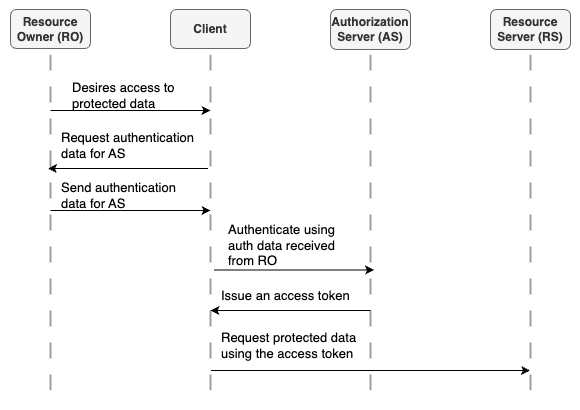
\includegraphics[width=0.75\textwidth]{pic/resource_owner_password_credentials_grant.png}
	\unitlength=0.75mm
	\special{em:linewidth 0.4pt}
	\linethickness{0.4pt}
	\caption{Resource Owner Password Credentials Grant}
	\label{fig:resource_owner_password_credentials_grant}
\end{figure}
	

\subsubsection{Client Credentials Grant}
The client credentials grant must only be used by confidential clients
interacting with each other. This means the clients have the ability to
securely store a secret, which is only accessible by themselves. A common
use-case for this scenario would be machine-to-machine interactions. This grant type is meant for clients to access their own resources as is the case in micro-service architectures. As depicted in figure \ref{fig:client_credentials_grant} the client authenticates at the authorization
server with its client secret and receives an access token, to authenticate at the resource provider. This means that the resource provider does not need to verify client secrets, but instead only needs the capability to verify access tokens. This fact is useful for practical reasons, as a resource provider could reuse the implementation of access tokens for other grant types it is offering.
\cite[Sec. 4.4.]{hardt2012rfc}

\begin{figure}[ht]
	\sffamily\footnotesize
	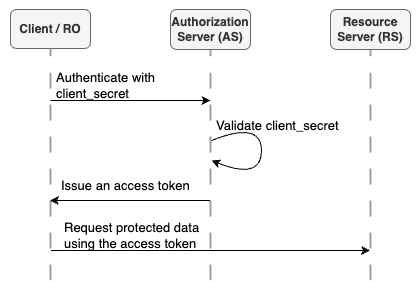
\includegraphics[width=0.6\textwidth]{pic/client_credentials_grant.png}
	\unitlength=0.75mm
	\special{em:linewidth 0.4pt}
	\linethickness{0.4pt}
	\caption{Client Credentials Grant}
	\label{fig:client_credentials_grant}
\end{figure}

\subsubsection{Device Authorization Grant}
Introduced in RFC8628 the device authorization grant is meant to be used for
devices, that lack a user agent like a web browser or do not offer a convenient
way of entering text \cite{denniss2019oauth}. In this grant type the client is
not mainly interacting through a user agent like a web browser anymore, but instead is using a device authorization endpoint at authorization provider directly to initiate an authorization request. The client, then instructs the user to open a webpage on a secondary device to complete the authorization process using a displayed code for verification of the session. This OAuth flow still requires the involved devices to use HTTP for communication, which in general is not a feasible solution for many IoT-devices. A solution for the popular IoT-protocol CoAP is proposed by Chung et al. 

\begin{figure}[ht]
	\sffamily\footnotesize
	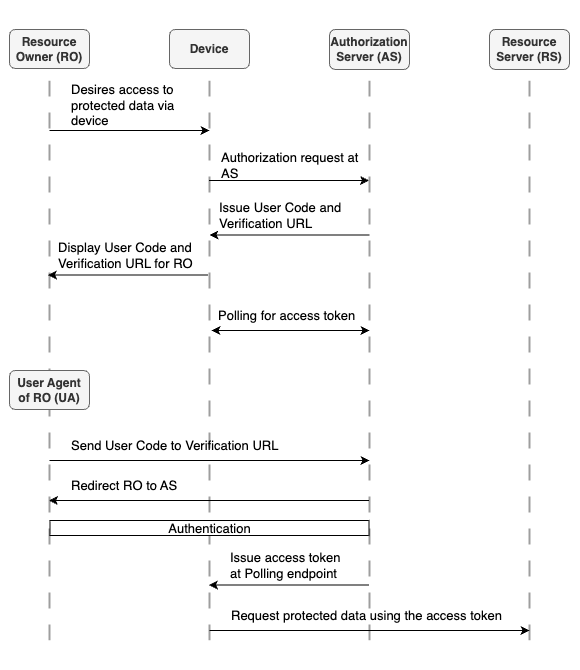
\includegraphics[width=0.75\textwidth]{pic/device_authorization_grant.png}
	\unitlength=0.75mm
	\special{em:linewidth 0.4pt}
	\linethickness{0.4pt}
	\caption{Device Authorization Grant}
	\label{fig:device_authorization_grant}
\end{figure}

\subsubsection{Other grant types}
There are several more grant types, which got introduced to the OAuth standard
over time, which are listed below, but are out of scope for this work: 

\begin{itemize}
	\item Refresh Token Grant
	\item JWT Bearer Grant
	\item UMA Grant
	\item SAML 2.0 Bearer Grant
	\item Token Exchange Grant
\end{itemize}

\subsection{Open ID Connect}
Open ID Connect (OIDC) is a layer on top of OAuth 2.0, introduced in 2014 by a combination of researchers and companies like Google, Microsoft and Salesforce, which form the OpenID group. The main focus of Open ID Connect is authentication, which means identifying a user but not authorizing the user. OIDC flows use a particular OAuth scope, which is called "openid", an extra token, the "ID token", which is a JWT token containing the identifying information about the user, which are called claims. The claims can be used to retrieve more information about the user at the OpenID provider, or the information can be directly part of the initial ID token, so OpenID adds the authentication to the already provided Authorization capability of OAuth. For OIDC, the same grants are used as for OAuth, but in the context of OIDC, they are often referred to as flows \cite{li2016analysing} \cite{sakimura2014openid}.

\subsection{The Future: OAuth 2.1}
OAuth 2.1 will be the next version of OAuth. There is currently one draft available at the IETF \cite{ietf-oauth-v2-1-09}. The main intent of this draft is to consolidate the various extensions to OAuth introduced in the last years. It simplifies the core document for OAuth 2.0 and omits outdated features because of new browser capabilities, which came over the last years and allow for more secure interactions. Below is a list of significant changes:
\begin{itemize}
	\item The Implicit Grant gets omitted
	\item The Resource Owner Password Credentials Grant gets omitted
	\item PKCE is required for the Authorization Code Grant
	\item Redirect URIs must be compared with exact string matching, so pattern matching is completely disallowed
	\item Access tokens must not be transported in a Request-URI in any case (which also makes the Implicit Grant impossible
\end{itemize}

In conclusion, the draft for OAuth 2.1 picks valuable features of existing standards for OAuth to require them and omits outdated features, intending, on the one hand, to simplify the OAuth landscape and, on the other hand, get rid of insecure features of the past.

\section{Intrusion Detection System}
An intrusion is any malicious behavior with the intention to damage or take control of an information system. All primary protection goals of information security, like confidentiality, integrity and availability, can be the target of an intrusion. A method to harden systems against intrusions is using intrusion detection systems (IDS), which monitor all traffic, events or actions of a system to detect when malicious actions are executed so the system's owner, the administrator or the system itself can take immediate action on intrusion attempts. If the intrusion detection system takes action to prevent intrusions, it is called an \emph{Intrusion Detection and Prevention System (IDPS)} \cite{scarfone2010intrusion}. There are several taxonomies for intrusion detection system types. For example, \cite{Liao2013IntrusionDS} categorized IDS into five categories: Statistics-based, Pattern-based, Rule-based, State-based, and Heuristic-based, referring to the methodology of detection the IDS is using. \cite{khraisat2019survey} build on top of that approach to further specify an overall taxonomy for IDS. The definition of Intrusion detection systems is based on the taxonomy summarized by these researchers.

\subsection{Distinction by input data}
Generally, when categorizing Intrusion Detection Systems by environment or input data, there are two types to distinguish them. 
\emph{Host-based Intrusion Detection Systems (HIDS)} and \emph{Network-based Intrusion Detection Systems (NIDS)}.
\subsubsection{Host-based Intrusion Detection System}
HIDS monitor all data concerning a host system, like operating system events, host firewall logs or application-specific logs. They can detect specific attacks on the system level without using network logs.
\subsubsection{Network Intrusion Detection System (NIDS)}
NIDS monitor network traffic, which is acquired by packet capture tools and other network data sources. One challenge of Network Intrusion Detection Systems is often the large amount of data that needs to be analyzed in high-bandwidth networks, which demands high computing capabilities.

\subsection{Distinction by detection characteristic}
When distinguishing types of intrusion detection systems by the way they operate, there are two categories: Signature-based (SIDS) and Anomaly-based (AIDS).

\subsubsection{Signature-based Intrusion Detection System}
Signature-based IDS utilize databases of fingerprints of already known attacks. These databases are called knowledge databases. A fingerprint could be, for example, a hash value of an executable malware file. A HIDS could compare any file an operating system executes against the knowledge database to detect the specific malware. The same concept also works for NIDS, e.g., when scanning mail attachments transferred via SMTP. The main advantage of SIDS is that they rarely produce false positive alerts when identifying intrusions. Their downside is that they cannot detect unknown attacks.

\subsubsection{Anomaly-based Intrusion Detection System}
The core concept for Anomaly-based IDS is to differentiate between usual and unusual behaviour. Unusual behaviour is identified as an intrusion. There is a variety of techniques that AIDS can use to achieve the goal of differentiating typical and malicious behaviour. One possibility is creating a statistical model over the data and filtering out events with a low probability. 
Another approach is to use machine learning techniques. Unsupervised learning methods, like clustering, on the one hand, are very similar to the statistical approach because the goal is again to sort out rare occurrences in small clusters. Supervised learning methods, on the other hand, create a model of usual behaviour in a training phase with labelled data to test any new input of unknown data if it is classified as malicious. 
An additional way for Anomaly-based IDS is the knowledge-based method. With this method, knowledge is applied to the detection in the form of rules to identify any behaviour that breaks those rules as an intrusion. These rules can stem from knowledge about a network protocol or any other system behaviour.

\subsection{zeek IDS}
\emph{Zeek} formerly known as \emph{bro}, as a reference to George Orwell's 1984 as a ``reminder that monitoring comes hand in hand with the potential for privacy violations'' \cite{zeek2023} is an open source network intrusion detection system. The first version of \emph{bro} was released in 1995 by the Lawrence Berkeley National Laboratory. In 2018, the project was renamed to \emph{zeek}. The system is often used for network security monitoring to detect and analyze suspicious behavior in network traffic. Its architecture consists of two major components, as displayed in Figure \ref{fig:zeek_architecture}. The first component is the \emph{event engine}, which refines the incoming network traffic into higher-level events without doing any analysis. It processes the traffic through different subcomponents, identifying protocols, file types, and, e.g. TCP connections at the link layer. The second component is the \emph{policy script interpreter}, which runs different event handlers to analyze the events. These event handlers are built in their own scripting language, but adaptors to public programming languages also exist and are applied in this work.

\begin{figure}[ht]
	\sffamily\footnotesize
	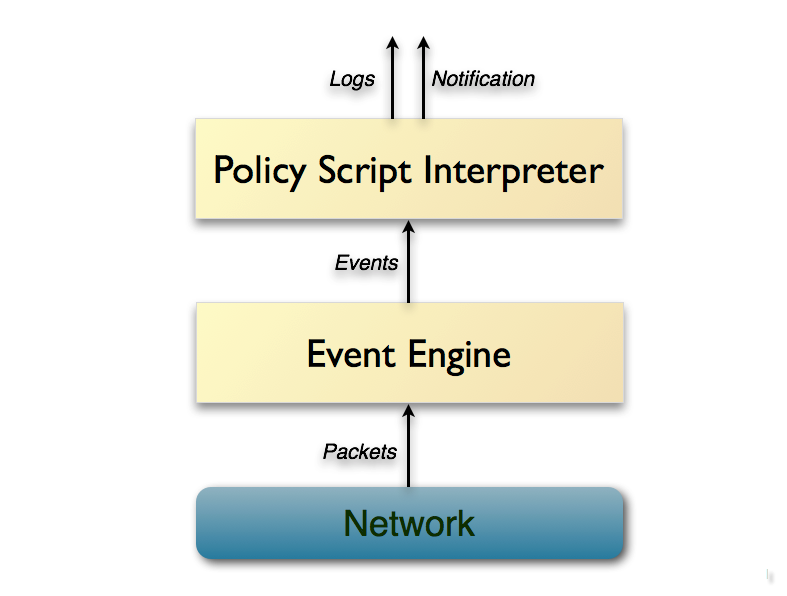
\includegraphics[width=0.75\textwidth]{pic/zeek_architecture.png}
	\unitlength=0.75mm
	\special{em:linewidth 0.4pt}
	\linethickness{0.4pt}
	\caption{Architecture of zeek \cite{zeek2023}}
	\label{fig:zeek_architecture}
\end{figure}

\section{Algorithms}
The algorithms applied in the experimental part of the work serve different purposes in the experiment chain described in Chapter \ref{chap:experimental_analysis}. These algorithms are essential for following along with the experimental approach. Therefore, this section starts by describing the technique for encoding the textual network data to numerical data. It follows up by illustrating the inner workings of two clustering algorithms applied to the encoded data at the end of the experiments.


\subsection{Word2Vec}
\emph{Word2Vec} introduced in 2013 by Mikolov et al. is a technique in natural language processing to convert words into embeddings. An embedding is a vector carrying a semantic to represent a word as a numerical value to enable the usage of words in algorithms requiring numerical inputs. In the case of \emph{Word2Vec}, the idea is that words hold similarities based on their surrounding words in a text corpus. This concept leads to words, which often stand close together in a text, receiving vectors that point in a similar direction. There are two models which are employed by \emph{word2vec}, the \emph{Continous Bag of words (CBOW)} model and the \emph{Skip-Gram} model. Both models have in common that they apply supervised learning techniques by training a neural network to predict relationships in text corpora. In both cases, the goal is to use the weights of the hidden layer after training as word embeddings instead of utilizing the neural networks for any predictions \cite{mikolov2013efficient} \cite{rong2014word2vec}.

\subsubsection{Continous Bag of Words (CBOW)}
The continuous bag of words model trains a neural network that predicts the word in the middle based on its surrounding words. An important hyperparameter for CBOW and Skip-Gram is the window size, which describes how many words surrounding a word are considered context. 
During training, the network receives combined one-hot-encoded vectors of surrounding words (e.g., averaging or summing them) in a tuple with the corresponding target word. When the training is completed at inference, the model gets context words as input and outputs a vector of probabilities for the predicted target word. But as mentioned above, the goal of word2vec is to extract word embeddings, which are the weights of the hidden layer of the neural network.

\subsubsection{Skip-Gram}
The skip-gram model uses the reverse strategy compared to the CBOW model. Instead of predicting a word by its surroundings, it trains a neural network that tries to predict the surroundings of a word. At training, the neural network receives word tuples of single context words and their corresponding target words one-hot-encoded. After fitting the network during inference, the model receives a one-hot-encoded word as input and produces a probability distribution over the vocabulary, which stands for the probability of a word being a surrounding word for the input. Again, in the case of word2vec, this supervised learning approach is only applied to retrieve the weights of the hidden layer as word embeddings, as word2vec is used for non-labelled data. In their research, Mikolov et al. state that skip-gram is feasible for small data sets and even considers rare occurrences of words well. In contrast, CBOW is faster in training with large datasets and better at capturing the semantics of high-frequency words. 

\subsection{k-Means Clustering}
In the field of data analysis, finding patterns and anomalies in data sets is a ubiquitous challenge. Grouping data into different clusters can be an approach to reveal useful features or meanings from the data. One common technique for clustering is k-means clustering. There are different flavors of k-means algorithms, but one of the most common k-means algorithms and the one applied in this work is Lloyd's k-means algorithm \cite{wilkin2007kmeans}. 
\subsubsection{Lloyd's k-Means clustering}
The general goal of the algorithm is to group data by similar features into a fixed amount of clusters. The algorithm achieves this by finding $k$ \emph{centroids} $\mu_1, \mu_2 ... \mu_k \in \mathbb{R}$. The clusters are then based on the centroids so that every point $x$ of the n-dimensional dataset ${x_1 ... x_m}$ gets assigned to the centroid with the lowest Euclidean distance. In order to find the centroids, the algorithm's approach is an iterative process described in figure \ref{fig:kmeans}. In the beginning, $k$ (defined by the number of clusters) random centroids are chosen. Then, the clusters are created by calculating the minimum Euclidean distance from every point of the dataset to the centroids: $\arg\min_j \|x_i - \mu_j\|^2$. In the next step, the centroids are recalculated by finding the points in the center of the clusters: $\mu_j = \frac{1}{|\mu_j|} \sum_{x_i \in \mu_j} x_i$. The two steps of creating the clusters based on the centroids and calculating the center point of the new clusters are repeated until the centroids converge or a definition for a fixed amount of iterations is given \cite{piech2013kmeans} \cite{lloyd1982kmeans}.



\begin{algorithm}
	\label{fig:kmeans}
	\caption{Lloyd's K-Means Algorithm}
	\begin{algorithmic}[1]
		\State \textbf{Input:} Data set $X = {x_1 \ldots x_m}$, number of clusters $k$
		\State \textbf{Output:} Cluster centroids $\{\mu_1, \mu_2, \ldots, \mu_k\}$
		\State Randomly choose $k$ centroids ${\mu_1 \ldots \mu_k}$ 
		\Repeat
		\For{each data point $x_i$}
			\State Assign $x_i$ to the cluster with the nearest centroid: $\mu_i = \arg\min_j \|x_i - \mu_j\|^2$
		\EndFor
		\For{each cluster $j$}
			\State Calculate new centroid $\mu_j$ as the center of all points assigned to cluster $j$ for every cluster: $\mu_j = \frac{1}{|\mu_j|} \sum_{x_i \in \mu_j} x_i$
		\EndFor
		\Until{New centroids don't change anymore or a fixed number of iterations was given}
	\end{algorithmic}
\end{algorithm}

\subsection{Self-Organizing Maps}
A Self-Organizing Map (SOM) is an unsupervised machine-learning algorithm that aims to reduce the dimensions of high-dimensional data. SOMs were introduced in 1990 by the Finnish engineer and senior member of the IEEE Teuvo Kohonen. As described in the initial publication, Self-Organizing Maps not only help with dimension reduction but also "One novel result is that the self-organization process can also discover semantic relationships in sentences". This aspect, in particular, is one reason the algorithm is applied in fields other than data visualization as well, like natural language processing and intrusion detection. At its core, a Self-Organizing Map is based on an artificial neural network that is trained using competitive learning. The network's input layer usually has many more dimensions than the output layer, which aligns with the algorithm's goal to reduce the dimensions of data. Then, there is an inner layer called the Kohonen Layer, a grid of neurons with the desired output's dimensions. This layer of neurons gets initialized at random in the beginning. The training process now works as follows:
\begin{enumerate}
	\item An input vector of the sample high-dimensional data gets randomly chosen. The neuron in the Kohonen layer, whose weight is most similar to the input vector, gets chosen by calculating the Euclidean distance: $$D(w, x) = \sqrt{\sum_{i=1}^{N} (w_i - x_i)^2}$$ for weight vector $w$, input vector $x$ for $N$ dimensions. The weight vector, which is chosen this way, is called the \emph{winner} or the \emph{Best Matching Unit (BMU)}.
	\item A neighborhood function gets applied to the BMU, influencing the weights of neighboring neurons. The neighborhood function is most often a Gaussian decay function: $$h(r, t) = \exp\left(-\frac{2\sigma^2(t)}{\|r\|^2}\right)$$ where $\|r\|^2$ is the Euclidean distance between the BMU and the neighbor, $t$ is the time (or iteration amount), which has passed and $\sigma^2(t)$ is the neighborhood radius, which decreases over time. This formula leads neurons near the BMU to be updated more heavily in the early stages of the training.
	\item The weights of the Kohonen layer are updated for multiple iterations to resemble the input vectors in the end. The output is the weights of the Kohonen layer, which have been reduced to the desired lower dimension.
\end{enumerate}
\chapter{Related Work}
\label{chap:related_work}
This chapter presents important research in the realm of OAuth security and intrusion detection using similar techniques as proposed in this work. As this thesis first builds a strong foundation in OAuth threats, Section \ref{sec:oauth_security_research} starts by showcasing important publications in the realm of theoretical security of the OAuth 2.0 standard. It then proceeds to present a recent study on practical implementations of OAuth, which was already mentioned briefly in the introduction

Section \ref{sec:anomaly_based_intrusion_detection} continues with examples of related work, which utilize similar techniques to the ones applied in this work, but in different contexts or based on different dataset approaches.

\section{OAuth Security Research}
\label{sec:oauth_security_research}
In the area of OAuth security, a lot of research focuses on analyzing implementations of the OAuth standard in practice. Surveys scanning public OAuth providers for vulnerabilities exist \cite{philippaerts2022oauch}, as well as analysis of OAuth flows using finite state machines \cite{munonye2022machine}. However, there are publications by one research group, that focus on the OAuth standard itself, which is presented in  Section \ref{subsec:fks_model}, because it had an important impact on the OAuth 2.0 standard itself.

\subsection{Theoretical Security Analysis of OAuth}
\label{subsec:fks_model}
Security research on the OAuth standard has been conducted since its beginnings. Impactful research that unveiled security issues in the definition of OAuth 2.0 is the work by Fett et al. \cite{fett2016comprehensive}, who constructed a theoretical \emph{Dolev Yao}-style model called the FKS model and extended that model with OAuth2 capabilities. On the one hand, the FKS model mimics web standards, like HTTP/1.1 and HTML5. On the other hand, it simulates entities like browsers, including the concept of windows, documents, iframes, complex navigation rules, DNS servers, web servers, and web and network attackers. The FKS model puts entities as processes into practice, while the communication through standards is modeled via events between the processes. For OAuth 2.0, the researchers' goal is to reveal security flaws in the most secure implementation of the standard regarding all publicly known security considerations while modeling the four grant types: \emph{implicit grant}, \emph{authorization code grant}, \emph{resource owner password credentials grant}, and \emph{client credentials grant}. The central methodology of Fett et al. is to prove the security of the OAuth standard using their formal language, in which the standard is modeled, to find the flaws breaking the security proof. Following this methodology, the researchers uncovered four new threats in the  OAuth standard, with the impact that the OAuth working group of IETF added these threats and their countermeasures to the official document for security best practices for OAuth \cite{lodderstedt2020oauth}.

\subsection{Analysis of OAuth implementations}
Through research like the one mentioned in Section \ref{subsec:fks_model} by Fett et al. and the continuous work by the OAuth working group of the IETF, the OAuth standard gets enriched with several suggestions for improving the security of OAuth implementations. However, because OAuth is such a complex protocol, implementation flaws still arise, even concerning already-known threats. A recent study by Philippaerts et al. implemented an audit tool called ``OAuch'' to test the coverage of countermeasures against known threats for OAuth. It revealed that 97 of 100 popular identity providers (OAuth and Open ID Connect) leave at least one common threat completely unmitigated. The researchers also found that, on average, OAuth identity providers, in particular, did not implement 34\% of the security specifications suggested by the OAuth working group \cite{philippaerts2022oauch}. This work again shows the importance of awareness of the threat landscape when implementing and operating an OAuth provider or an OAuth client.

\section{Anomaly-based Intrusion Detection}
\label{sec:anomaly_based_intrusion_detection}
In the realm of intrusion detection, anomaly-based intrusion detection is a popular research topic, as this type of detection bears one important advantage. Anomaly-based intrusion detection possibly detects unknown attacks in network traffic. Over the last two decades, research in this area has been conducted on benchmark datasets like the \emph{KDD’99} dataset \cite{kdd1999} and updated versions of it. Even though this work uses a self-simulated dataset, because of the lack of existing OAuth intrusion network data, techniques applied in such research can be transferred to the scenario of this work. Relevant research for these techniques is showcased in the following sections.

\subsection{Word embeddings for feature extraction}
One issue to overcome, when working with data logs is to extract relevant features and convert them into a form, that is digestible for machine learning algorithms. Especially textual data, which may hold semantic meaning poses a challenge in that regard. The research by Corizzo et al. \cite{corizzo2020feature} focuses exactly on tackling this issue, by proposing methods, where raw system calls get encoded by different NLP algorithms. The researchers tested their methods on three different datasets and concluded that an approach combining Word2Vec and TF-IDF performs the best. As visualized in Figure \ref{fig:w2v_feat_extr} even just applying Word2Vec performed in the same area of results as the combination with TF-IDF. Even though the work by Corrizzo et al. concludes that the results are not vast enough, it shows that there is potential in this technique to carry out intrusion detection tasks.

\begin{figure}[H]
	\sffamily\footnotesize
	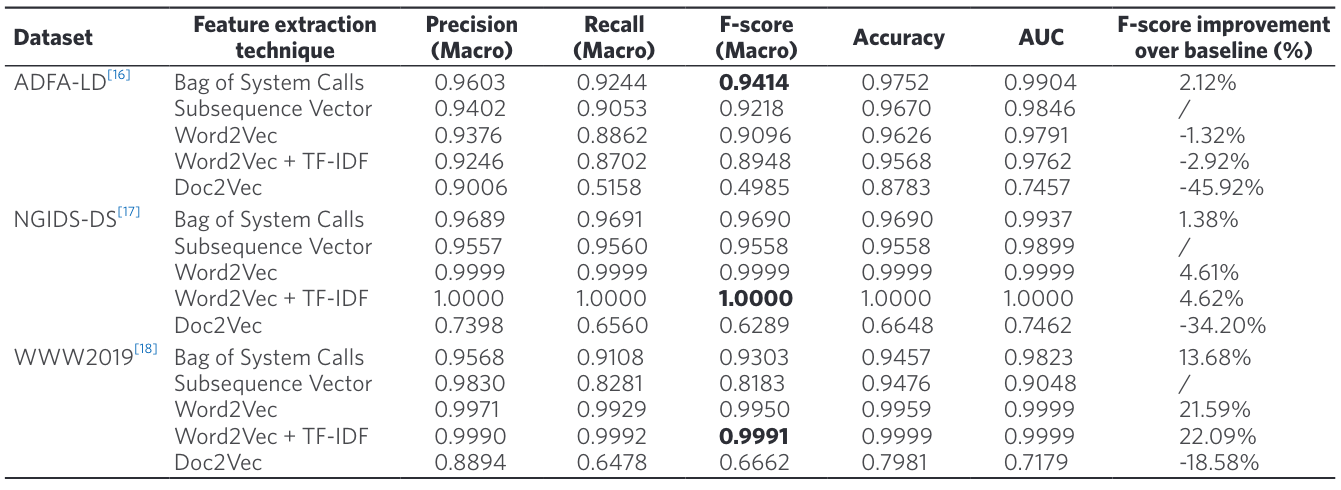
\includegraphics[width=1\textwidth]{pic/w2v_feat_extr.png}
	\unitlength=0.75mm
	\special{em:linewidth 0.4pt}
	\linethickness{0.4pt}
	\caption{Results of applying different NLP techniques for feature extraction on three different datasets of Host-based intrusion data \cite{corizzo2020feature}}
	\label{fig:w2v_feat_extr}
\end{figure}


\subsection{K-Means and intrusion detection}
\label{subsec:k_means_intrusion_detection}
Clustering algorithms, like k-Means, have their place in the anomaly-based intrusion detection research landscape for several years. Earlier research focuses on solely applying these algorithms to filter out anomalous traffic by calculating cluster centroids using k-means and measuring the distance from every datapoint to every centroid to determine outliers for anomaly detection \cite{munz2007traffic}. The research by Nalavade et al. \cite{nalavade2014} is an example of applying the k-Means algorithm for network intrusion detection again using the famous \emph{KDD`99} dataset \cite{kdd1999}. The researchers preprocess the data by determining features, that hold more relevance than others and increasing their weights for the clustering, by altering their distance metric during clustering. The results depicted in Figure X show that Navalde et al. had some success detecting certain types of attacks like Denial of Service. 

\begin{figure}[H]
	\sffamily\footnotesize
	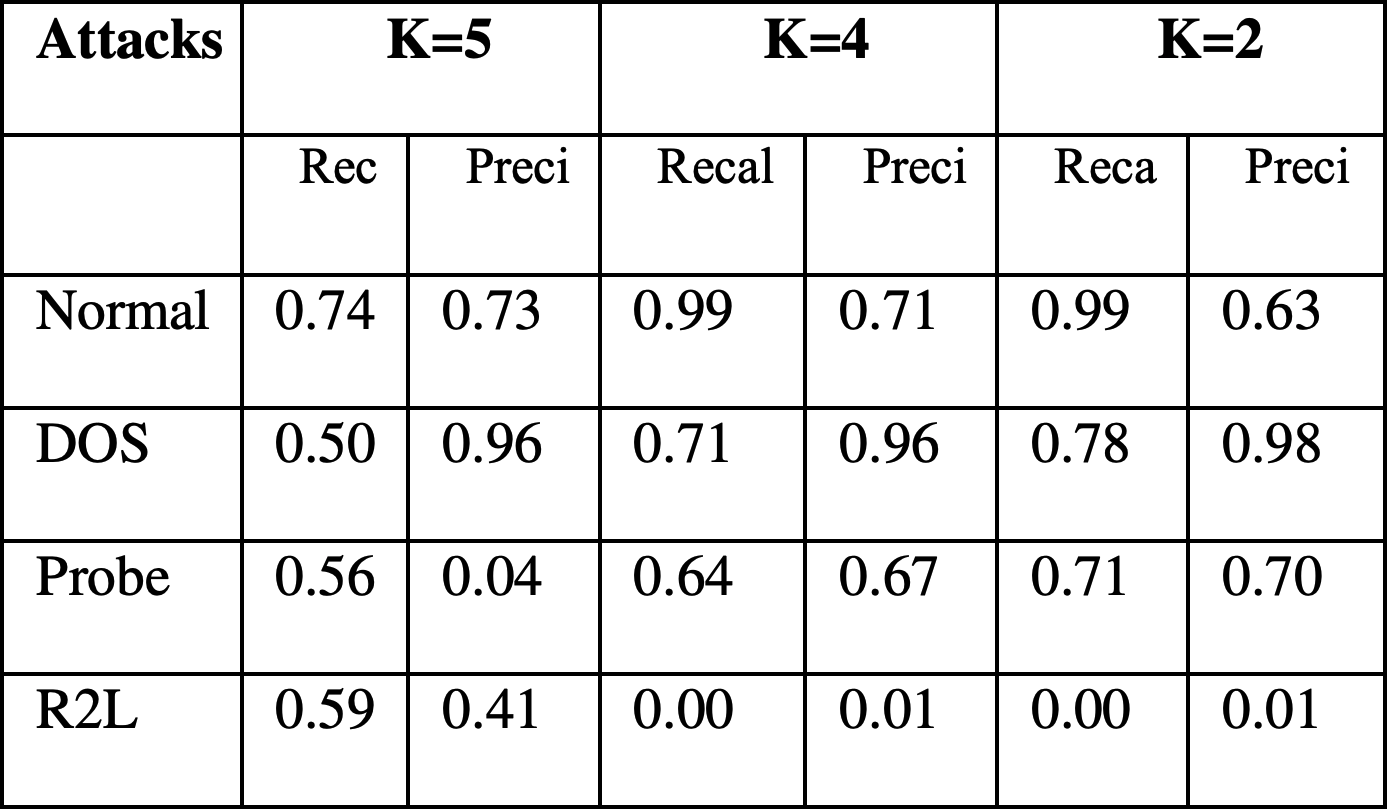
\includegraphics[width=0.5\textwidth]{pic/navalde_k_means.png}
	\unitlength=0.75mm
	\special{em:linewidth 0.4pt}
	\linethickness{0.4pt}
	\caption{Results by Navalde et al. applying k-Means for different cluster sizes $K$ to the KDD`99 dataset after pre-processing the data for intrusion detection \cite{nalavade2014}}
	\label{fig:k_means_navalde}
\end{figure}


\subsection{Self-organizing Maps and intrusion detection}
Besides k-Means other clustering approaches are frequently researched for intrusion detection. One of these other clustering algorithms is the Self-Organizing Maps algorithm. A survey by Qu et al. \cite{qu2021survey} provides a taxonomy of different SOM approaches for network intrusion (see Figure \ref{fig:som_taxonomy}). The researchers present generally three main categories, where static SOMs are not able to adapt dynamically to new input data, whereas dynamic SOMs have this capability. The hybrid SOMs are a combination of SOMs with any other technique. One example of such a hybrid SOM is the combination of SOM and k-Means, which improves the overall performance in intrusion detection on the KDD`99 dataset (see Figure \ref{fig:som_kmeans}) based on the results of different studies gathered by the survey. Figure \ref{fig:som_kmeans} also shows that the results for k-Means without SOM are significantly better than the results presented in section \ref{subsec:k_means_intrusion_detection}. This further emphasizes that the preprocessing of the data is a very important step for intrusion detection.

\begin{figure}[H]
	\sffamily\footnotesize
	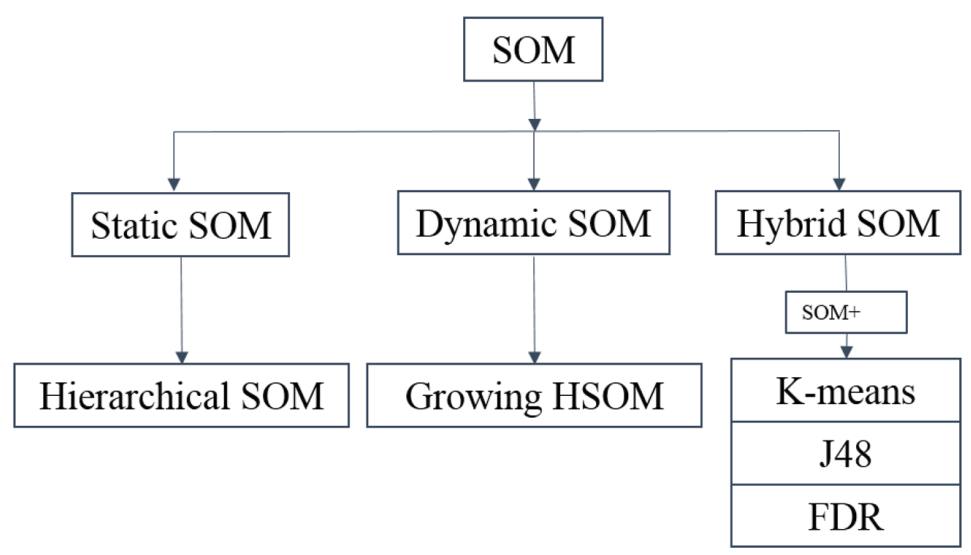
\includegraphics[width=0.5\textwidth]{pic/som_taxonomy.png}
	\unitlength=0.5mm
	\special{em:linewidth 0.4pt}
	\linethickness{0.4pt}
	\caption{Taxonomy of different approaches for implementing Self-Organizing Maps \cite{qu2021survey}}
	\label{fig:som_taxonomy}
\end{figure}

\begin{figure}[H]
	\sffamily\footnotesize
	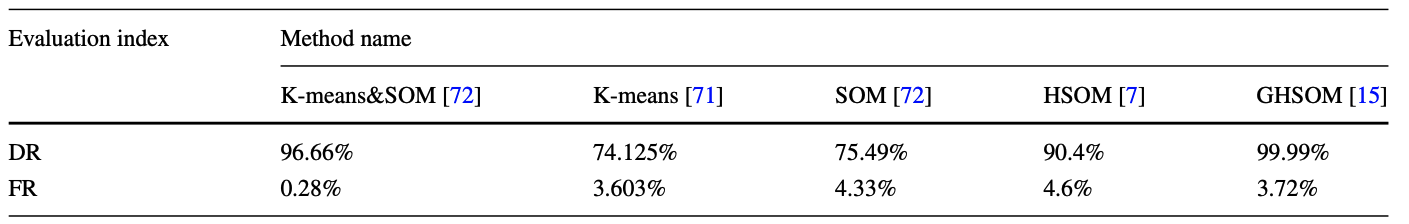
\includegraphics[width=0.9\textwidth]{pic/som_kmeans.png}
	\unitlength=0.5mm
	\special{em:linewidth 0.4pt}
	\linethickness{0.4pt}
	\caption{Results of different research, applying SOM methods for intrusion detection on the KDD`99 dataset (\emph{DR=detection rate, FR=false positive rate}) \cite{qu2021survey}}
	\label{fig:som_kmeans}
\end{figure}


\chapter{OAuth Threat Landscape}
\label{chap:oauth_security}

This chapter presents an overview of the currently known threat landscape when using the OAuth framework. Section \ref{sec:oauth_threats_and_vulns} elaborates on every threat separately. The list is mainly based on the current draft for security best practices for OAuth from the OAuth task force at IETF \cite{lodderstedt2020oauth} and is enriched with examples and further explanations.

Section \ref{sec:oauth_countermeasures} showcases different countermeasures, which can be applied to mitigate the presented threats. 

Finally Section \ref{sec:oauth_classification} presents two schemas to classify the OAuth threats and countermeasures.

\section{Threats}
\label{sec:oauth_threats}
Over the 11 years of the existence of OAuth 2.0, there has been always an effort to learn about threats and vulnerabilities, when applying the protocol. When the standard was introduced in 2012 browsers did not have the feature set they have today. This implies on the one hand, that new browser features could lead to new threats and on the other hand that new browser features could help mitigate older threats, which the standard of course could not foresee when it was created. An elaborate source for getting informing about the status of the OAuth threat landscape is the ongoing draft by the OAuth working group of IETF about the best current practice in OAuth security \cite{lodderstedt2020oauth}. As mentioned in Section \ref{subsec:fks_model} the draft is influenced by state-of-the-art research about OAuth security in a collaboration effort. This is the reason this section is mostly based on this draft and enriched with examples of other research work at appropriate places. Also every threat explained in this section receives an encoding in the form of \emph{T<number>} to reference them in later tables. These encodings can be found at the end of every paragraph.


\subsection[Insufficient Redirect URI Validation]{Insufficient Redirect URI Validation (T1)}
\label{threat:T1}
Authorization Servers need to whitelist redirection URLs in order to make sure, that an attacker cannot craft a hyperlink, which leads to the victim initiating an OAuth flow and sending the authorization code or token to an attacker-controlled domain. Some authorization servers may allow the usage of patterns in order to allow several domains at once. As well as the absence of any sort of whitelist mechanism even a pattern-matching functionality could lead to security problems. Among the possibility that a user is entering
patterns that are too broad and allow the usage of unintended redirect URLs, the attack surface includes issues with the URL parsing implemented by the authorization server as shown by Wang et al. \cite{wang2019make}. They presented several techniques to trick the parser into accepting unintended domain names, like using squared brackets for IPv6 parsing or the \emph{Evil Slash Trick}, where the parser does not treat a forward slash as a path
separator, while modern browsers do. Depending on the OAuth grant type in use this vulnerability leads to different possibilities to exploit it \cite{lodderstedt2020oauth}.


\subsubsection{Authorization Code Flow}
Using the example of the authorization code flow the threat of insufficient redirect URI validation can be exploited by crafting arbitrary redirect URIs in the following way:

\begin{enumerate}
    \item The attacker uses techniques like phishing to make its victim open an
        attacker-controlled webpage, which initiates an OAuth flow with the
        vulnerable authorization server.
	
    \item The request is crafted with a valid client ID (which is public
        information), ``code'' as response type and a malicious redirect URI,
        which leads to an attacker-controlled server again.
	
    \item If the user logs in at the authorization server, the authorization
        code now gets transmitted to the attacker's webpage, via the redirect
        URI.
	
    \item The attacker page can now use the received authorization code, to
        retrieve a token 
\end{enumerate}


\subsection[Credential Leakage via Referer Headers]{Credential Leakage via Referer Headers (T2)}
\label{threat:T2}
The Referer HTTP header is a potential attack surface. It can be utilized by a
malicious actor to capture query parameters, which are sent via the front
channel, like the state and the authorization code. The authorization code may
be used to redeem an access token before the victim retrieves it and the state
parameter oftentimes includes a CSRF token, which could potentially open up
vulnerabilities in other parts of the application as explained by Fett et al
\cite{fett2016comprehensive}.

\subsubsection{OAuth Client}
If a client renders third-party content, like advertisements in iframes or
images, before redeeming the authorization code for an access token an
attacker, who places these advertisements or images can capture the code via
the referer header and redeem it for an access token.

\subsubsection{Authorization Server}
At the authorization server, the state parameter could be leaked via the
Referer header, when third-party images or advertisements are being rendered on
the page. This may be an issue when the state contains a CSRF token as
explained by Fett at al \cite{fett2016comprehensive}.


\subsection[Credential Leakage via History Logs]{Credential Leakage via History Logs (T3)}
\label{threat:T3}
OAuth potentially transports sensitive data via the request-URI, like the access token, as is the case when the implicit grant is used or if other grant types optionally allow the transportation of access tokens or authorization codes via URI parameters. Therefore, a person accessing the user's browser can extract this sensitive data and try to replay it. The same threat is present when a logging server is present, for example, in a corporate network \cite{lodderstedt2020oauth}. Research about browser history security focuses mainly on accessing information about the victim's history by comparing cache timings if a page was visited \cite{bansalcache}. This type of threat is irrelevant in the OAuth context because an attacker would need to guess the access token, which the attacker could endeavor outside the browser history as well. However, recent studies on the security of browser extensions show that malicious browser extensions could access the browser history, or data could be leaked by utilizing vulnerable browser extensions \cite{eriksson2022}.

\subsection[Mix-Up Attack]{Mix-Up Attack (T4)}
\label{threat:T4}
In this attack, at least two authorization providers are involved. The target AP and the attacker AP. The OAuth standard allows the resource provider to interact with multiple authorization providers, one of which could be malicious, so the security for such interactions must also be provided. The attack is feasible for the implicit and authorization code grants and works similarly for both. Another precondition is that the resource owner registers the same redirect URI at both authorization providers, which is typical for Open ID Connect dynamic client registration \cite{hosseyni2023formal}. With these preconditions present, the attacker now waits until the target initializes an OAuth flow with the attacker AP. The attacker then intercepts the initialization request and exchanges the target AP with its attacker AP. When the target client gets redirected to the attacker AP, the target gets immediately redirected back to the target AP for authentication. At the same time, the client ID in the query parameters of the redirection URL gets replaced with the one registered at the target AP. Suppose the target user authenticates because it did not detect that it intended to authenticate at another AP. In that case, an authorization code gets issued to the client when the authorization code grant used. The client then proceeds to try to redeem an access token at the attacker AP, as the client still thinks that it initiated an OAuth flow with the attacker AP. The attacker can now use the received authorization code to redeem an access token at the target AP. \cite{fett2016comprehensive}

\subsection[Authorization Code Injection]{Authorization Code Injection (T5)}
\label{threat:T5} 
The precondition for an authorization code injection is that an attacker has
successfully stolen an authorization code. This can be accomplished in various
ways for example by tricking the user into installing a malicious browser
extension, using other vulnerabilities in a web app like open redirections, or
abusing proxy auto-configuration files \cite*{philippaerts2022oauch}.

In the case, that the client is using the authorization code flow the attacker
can use the stolen authorization code to fetch an access token before the
client does.

\subsection[Access Token Injection]{Access Token Injection (T6)}
\label{threat:T6}
This kind of attack describes the process of an attacker using a stolen access
token in a legitimate authentication flow, to impersonate the client. If the
implicit flow is available, the attacker can now start a new flow and simply
replace the access token in the authorization servers' response. This will
circumvent any CSRF protection, as there is no difference to a non-compromised
flow. \cite{lodderstedt2020oauth}


\subsection[Cross Site Request Forgery]{Cross Site Request Forgery (T7)}
\label{threat:T7}
This type of attack, often referred to by its abbreviation ``CSRF"", is about
the attacker executing a request in the name of the user, by tricking the user
into executing requests for the attacker including all required authentication,
or authorization information. The default OAuth protocol does not include
protection mechanisms against this type of attack. 

\subsection[PKCE Downgrade Attacks]{PKCE Downgrade Attacks (T8)}
\label{threat:T8}
If an authorization server is not implemented to require PKCE for all its
flows, it is susceptible to being vulnerable to PKCE downgrade attacks
\cite{philippaerts2022oauch}. Even if it is documented otherwise, attackers
might try to omit PKCE parameters, as the current OAuth 2.0 standard does not
require the usage of the PKCE extension \cite{hardt2012rfc}. 


\subsection[Access Token Leakage at the Ressource Server]{Access Token Leakage at the Ressource Server (T9)}
\label{threat:T9}
In the scenario that clients can dynamically connect to resource servers at runtime, as is the case in mail or banking applications, an attacker could create a malicious resource server and trick the user into sending valid access tokens for the target data to the malicious resource server. It could also be the case that the client application is misconfigured to send access tokens to a dynamically created resource server. Another vector for Access token leakage at the resource server is when the server itself gets compromised, so the attacker receives access tokens by analysing connections to the server itself \cite{lodderstedt2020oauth}.

\subsection[307 Redirect]{307 Redirect (T10)}
\label{threat:T10}
The OAuth standard does not specify which type of HTTP redirect should be implemented to redirect the user back to the client after the authentication at the authorization provider is successful. As the HTTP 307 redirect reuses the header and the body of the original request \cite{fielding1999rfc2616}, a malicious client could extract the username and password of the initial form submission action because it receives this data as part of the redirection \cite{fett2016comprehensive}.

\subsection[Client Impersonating Resource Owner]{Client Impersonating Resource Owner (T11)}
\label{threat:T11}
In the scenario that an authorization server allows for multiple grant types, including the client credentials grant and another typical grant like the authorization code grant, the threat of a malicious client impersonating a resource owner can be present in certain implementations. One example is when the authorization server allows for dynamic registration of clients, with the possibility of setting a client ID. A client could set its ID to the value of an identifying value of a resource owner. To build the example further, Open ID Connect uses a token's subject property to identify a user \cite{sakimura2014openid}. A client could use the subject value as its client ID. Improper implementations of resource servers, which do not distinguish between token types by grant type, could mistake an access token issued to a resource owner with a token issued to a client, which allows the malicious client to access the protected data of the resource owner \cite{lodderstedt2020oauth}.


\subsection[Authorization Server Redirecting to Phishing Site]{Authorization Server Redirecting to Phishing Site (T12)}
\label{threat:T12}
When the authorization server allows dynamic client registration, an attacker could create a valid client to which the authorization server could redirect. The attacker then crafts a malicious authorization request that will always fail by appending an invalid \emph{scope} value and then will redirect to the phishing site. An example of such a malicious authorization request is depicted in Figure \ref{fig:phishing_requests}. As the authorization attempt using this crafted URL is always invalid because of the \emph{scope}, the victim immediately gets redirected back to the site given by the \emph{redirect\_uri} parameter, which legally got enlisted through dynamic client registration. This site could be a copy of the valid login page to trick the user into entering its credentials. This way of phishing is very subtle as the domain of the phishing link is valid and known by the victim. The victim would need to identify that the \emph{redirect\_uri} query parameter is invalid and realize that it gets redirected to this URL after clicking on the link with the valid domain \cite{lodderstedt2020oauth}.


\begin{figure}[ht]
	\sffamily\footnotesize
	\url{https://valid-site.com/authorize?scope=invalid&redirect_uri=https://phishing-site.com/login&client_id=client_id_of_malicious_client}
	\special{em:linewidth 0.4pt}
	\linethickness{0.4pt}
	\caption{Phishing request}
	\label{fig:phishing_requests}
\end{figure}

\subsection[Unvalidated Redirects and Forwards]{Unvalidated Redirects and Forwards (T13)}
\label{threat:T13}
This type of vulnerability, known as \emph{Unvalidated Redirects and Forwards} (URF) as well as \emph{Open Redirect}, exists when a web application exposes redirection or forward capabilities to untrusted user input, for example, through query parameters. An attacker could generally utilize URF vulnerabilities to craft phishing links that are masked with valid, trustworthy domains \cite{wang2015urfds}. Especially in connection with OAuth, an attacker using an existing URF vulnerability in a client can potentially circumvent whitelists for redirection URIs, by masking the redirect to a malicious client with a valid client exposing an open redirect in the query parameter \cite{lodderstedt2020oauth}. Section \ref{threat:T12} describes a different attack aimed at masking a phishing attack utilizing a mechanism specific to OAuth that is similar to an open redirection at the authorization server and therefore a threat, which is introduced by the implementation of OAuth itself.

\subsection[Clickjacking]{Clickjacking (T14)}
\label{threat:T14}
As authorization providers authorize applications to access confidential data, they are susceptible to being targeted by clickjacking attacks. Clickjacking attacks trick users into performing clicks on elements on a web page the users did not intend to interact with, e.g., by overlaying invisible iframes. In the case of OAuth, an attacker could create a malicious application and register it at the authorization provider of the target. The attacker also prepares a webpage that tricks the user into clicking on an invisible iframe of the authorization provider. The iframe could contain the grant access step of allowing the malicious application to access the user's confidential data. If the user has an active session at the authorization provider, a single click is enough to fulfill this action \cite{gibbons2014security}. 


\section{Countermeasures}
\label{sec:oauth_countermeasures}
Addressing the issue of the ever-evolving threat landscape of OAuth several countermeasures have been established in a head-to-head race with the exploitations of vulnerable OAuth implementations. The countermeasures profit from the same circumstance of ongoing browser development as the threats. Countermeasures today can leverage new protection features, which were not present in the past. These countermeasures are also well documented by the OAuth working group of IETF \cite{lodderstedt2020oauth}. In this section, these common countermeasures are briefly explained. Again they receive an encoding at the end of their section's headline for later reference.

\subsection[Mandatory PKCE]{Mandatory PKCE (C1)}
\label{counter:C1}
As an extension to OAuth defined by RFC 7636, \emph{Proof Key for Code Exchange (PKCE)} is a technique to mitigate several OAuth threats \cite{bradley2015rfc}. The main problem PKCE solves for the authorization code grant is verifying that only the original client who started an OAuth flow receives the access token, so a stolen authorization code cannot just get exchanged with an access token by the entity who stole the code. Figure \ref{fig:pkce} shows the way PKCE works \cite{siriwardena_oauth_2020}:

\begin{enumerate}
	\item Initially, before the client redirects the resource owner\'s user agent to the authorization server, it generates a random string of length 43 at minimum, called the \emph{code\_verifier}. It then calculates the hash value of the code\_verifier and encodes it with base64 without padding. The hash algorithm in use should be one which is currently regarded as secure and known by the authorization server. The resulting value is called the \emph{code\_challenge}
	
	\item At redirection to the authorization server, the client appends the code\_challenge and the hashing algorithm, which it has used to create the code\_challenge to the redirection URL as query parameters.
	
	\item After successful authentication, the authorization server creates a record of code\_challenge and the corresponding authorization code it generates and sends back to the user agent. Alternatively, it may append the code\_challenge to the authorization code and create the record this way.
	
	\item When exchanging the authorization code for an access token, the client sends the code and the code\_verifier to the authorization server.

	\item The client compares the code\_verifier with the corresponding code\_challenge of the authorization code by calculating the unpadded base64 encoded hash value of the provided code\_verifier. Only the client who initially requested protected resources could possess the random value that matches the code\_challenge.
\end{enumerate}


The PKCE mechanism mitigates several threats and vulnerabilities, as shown in Table X. It mitigates credential leakage via referer headers (T2), as this attack aims in the case of the authorization grant to extract authorization codes after a redirect. Even with a stolen authorization code, an attacker does not know the code\_verifier and thus can not receive an access token. For the same reason, any kind of authorization code injection (T5), where the precondition is a stolen authorization code, would only be possible by knowing the code\_verifier. Protection against cross-site request forgery (T7) is also provided since an attacker could not trick a client into appending confidential data to the resources owned by the attacker, as the victim\'s client does not send the attacker\'s code\_verifier to the authorization server. Lastly, protection against PKCE downgrade attacks (T8) is ensured when the authorization server implements PKCE as mandatory.

\begin{figure}[ht]
	\sffamily\footnotesize
	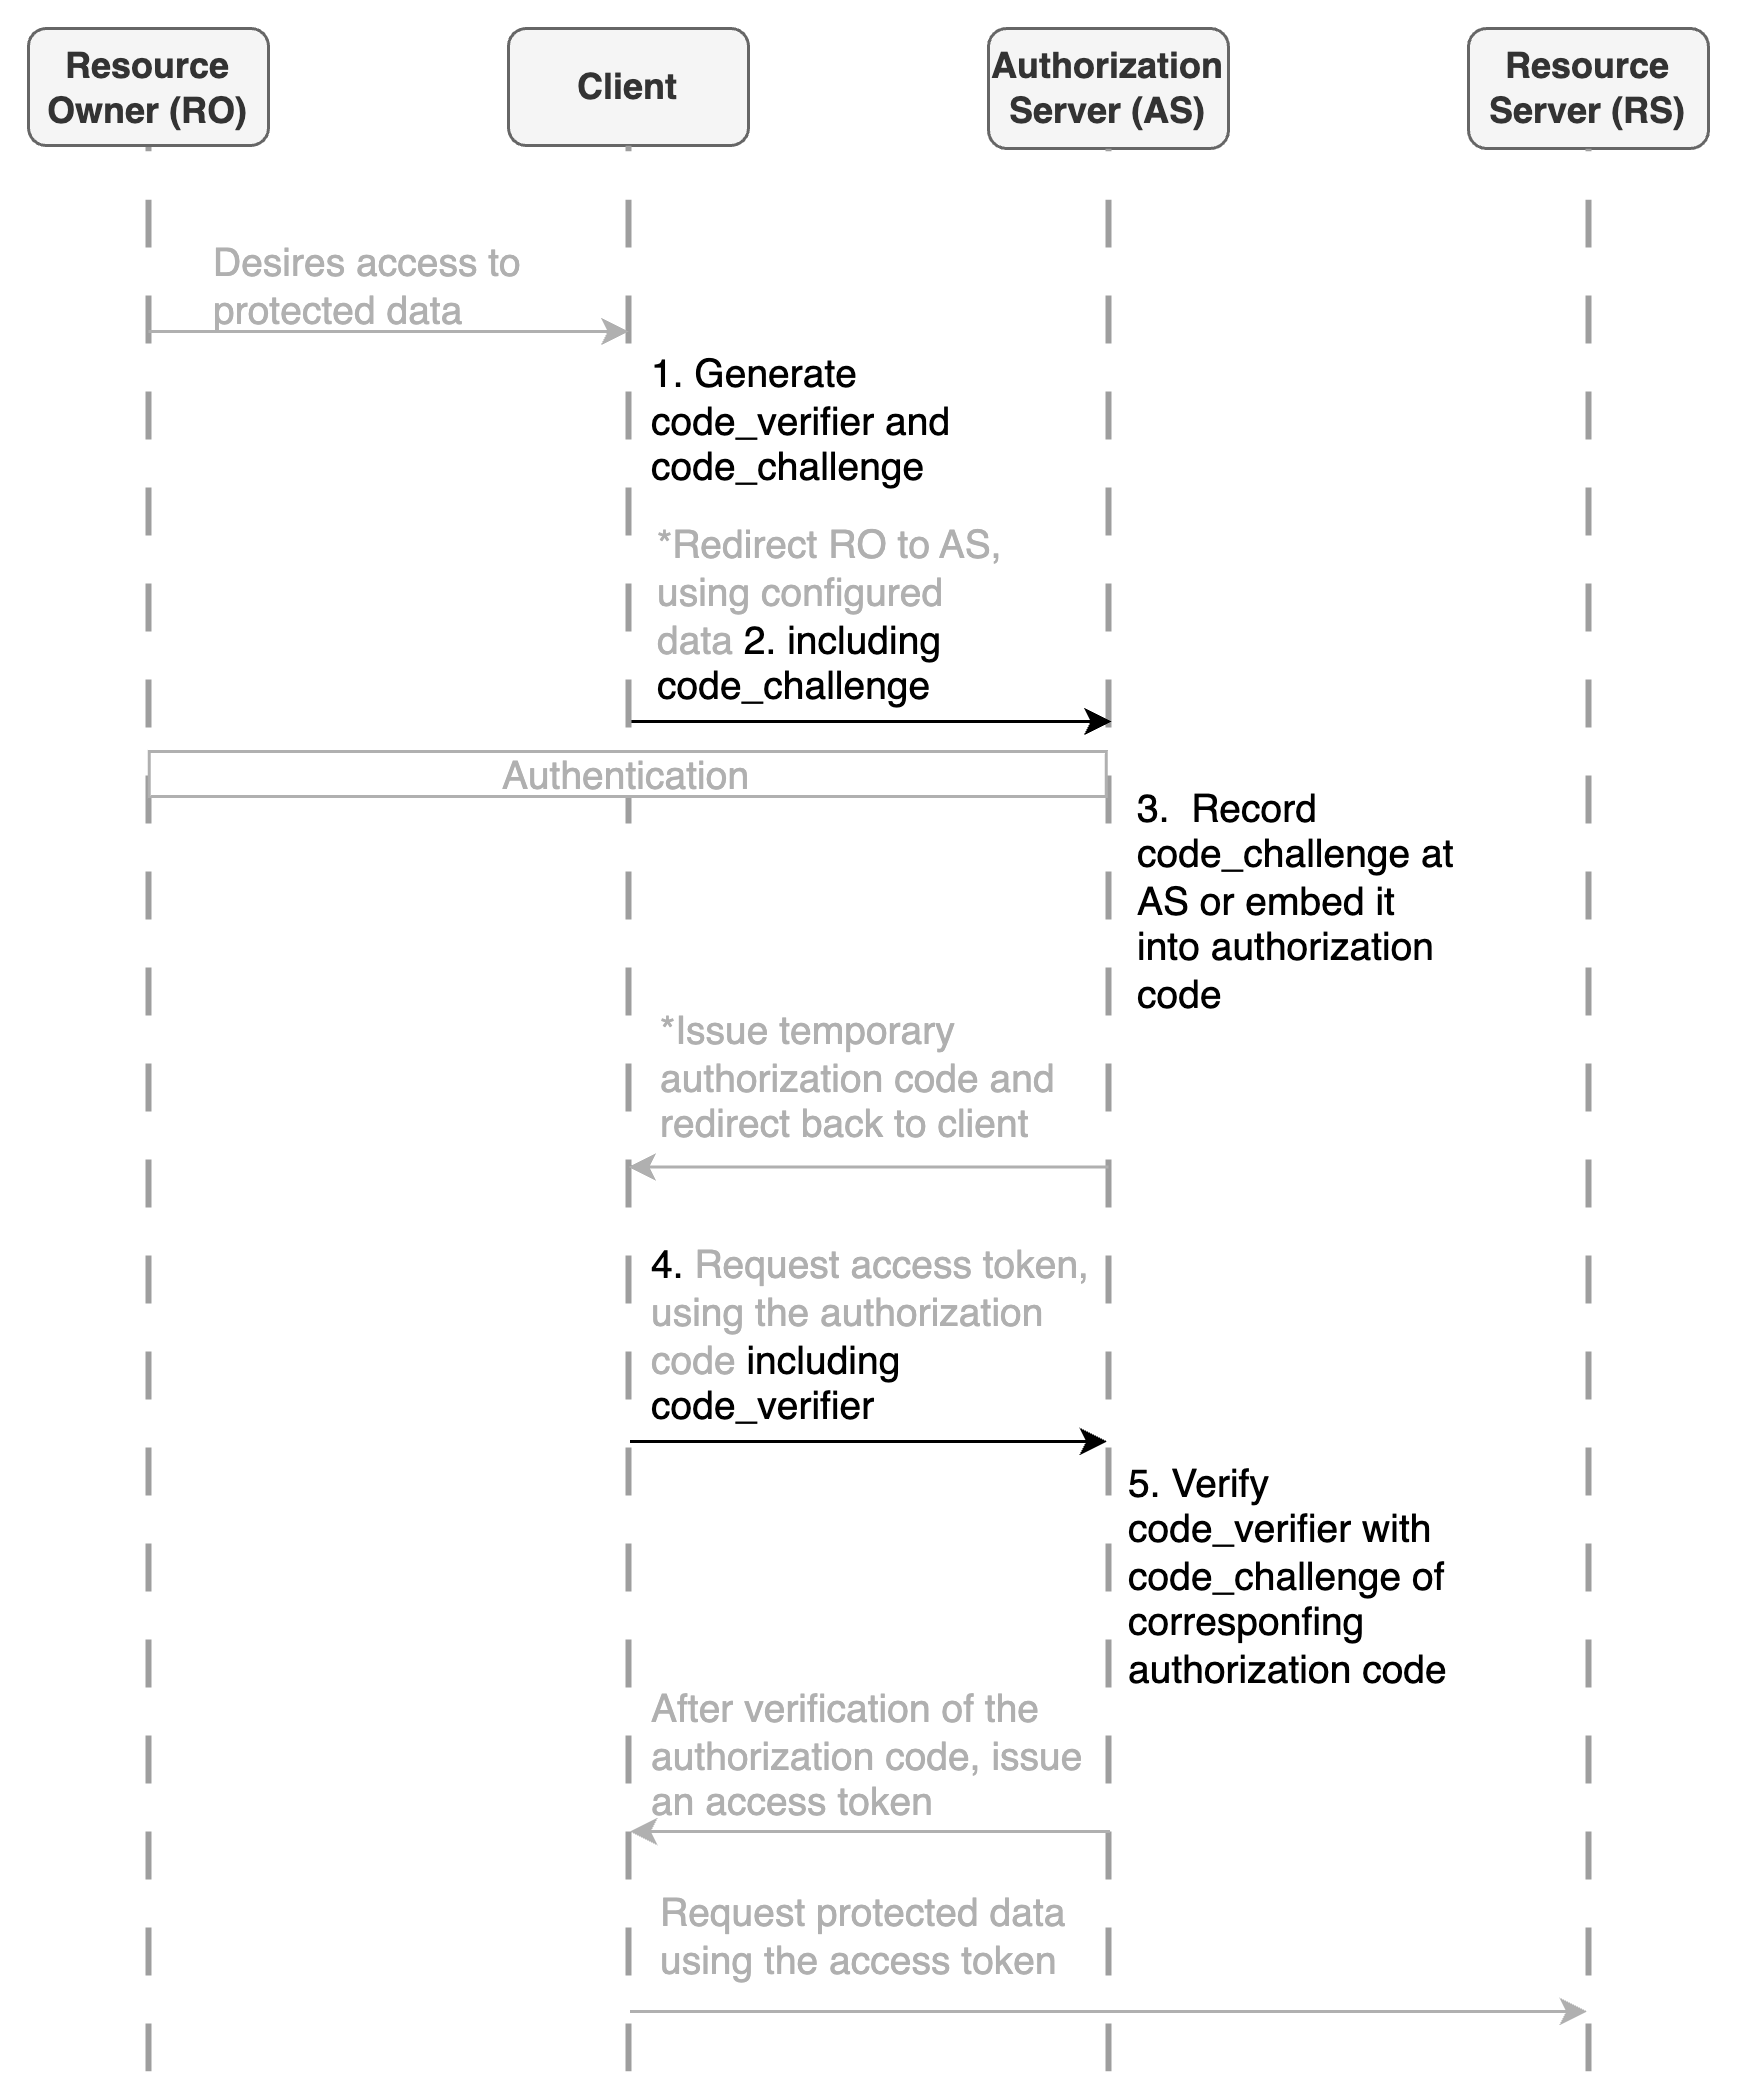
\includegraphics[width=0.75\textwidth]{pic/PKCE.png}
	\unitlength=0.75mm
	\special{em:linewidth 0.4pt}
	\linethickness{0.4pt}
	\caption{Authorization Code Grant with extension for Proof Key for Code Exchange}
	\label{fig:pkce}
\end{figure}

\subsection[Random value state]{Random value state (C2)}
\label{counter:C2}
Another method to protect against Cross-Site request forgery is by taking advantage of the state parameter the OAuth standard offers. When the client initiates an authorization request, it generates a random value of sufficient length, attaches it to the current session and sets it as the state parameter for the request. After authentication, the authorization server has to attach the previously received state parameter to the redirection URI as a query parameter. The client can now validate the received state value with the one it attached to its session earlier to ensure the redirection stems from the authorization flow it initiated \cite{ferry2015security}. When PKCE for the authorization code grant is already implemented, this measure does not add any benefit regarding CSRF protection \cite{bradley2015rfc}. In conclusion, the usages of state's main difference to PKCE is that the client knows that the received authorization code is connected to its initial authorization request before redeeming an access token with the code\_verifier, where the authorization server relates the client's requests to each other with the code\_challenge and the code\_verifier.


\subsection[Invalidation of access tokens]{Invalidation of access tokens (C3)}
\label{counter:C3}
The OAuth framework requires an authorization code to be redeemed only once for an access token. Therefore, an authorization code needs to be invalidated after its first usage. However, this does not stop an attacker from receiving an access token with a stolen authorization code before the valid user does it. The original OAuth standard recommends invalidating a previous access token if there was an attempt to receive an access token at least twice for the same authorization code \cite{hardt2012rfc}. Invalidation of access tokens if an authorization code gets redeemed twice helps mitigate the threats of credential leakage via referer headers (T2) and credential leakage via browser history (T3) \cite{lodderstedt2020oauth}, as for these threats, exposed authorization codes were already redeemed in most cases.
\todo{Auth code injection? Check table Mitigation responsibility}

\subsection[Simple string comparision]{Simple string comparision (C4)}
\label{counter:C4}
A technique to completely circumvent the threat of insufficient redirect URI validation (T1) is to disallow whitelisting redirect URIs using regular expressions. Instead, exact string comparison should be the way to allow redirections \cite{lodderstedt2020oauth}.

\subsection[Avoid usage of grant types]{Avoid usage of grant types (C5)}
\label{counter:C5}
Threats like credential leakage via referer headers (T2) or browser history (T3) can be avoided when the implicit grant is not used at all, as the access token would not be in the URI of a request. Access token injection (T6) using the implicit grant makes it easy for any attacker to circumvent CSRF protection through the state parameter (see Section \ref{counter:C2}) since, for the client, it does not make a difference what access token is used for the state check \cite{lodderstedt2020oauth}. For these reasons, the OAuth task force removed the implicit grant in the draft for OAuth 2.1 \cite{hardt2023rfc}. In the past the main benefit of the implicit flow was that it was possible to implement it for clients that did not utilize cross-origin resource sharing (CORS). CORS was finalized in 2014 by the W3C and superseded by the fetch standard afterwards \cite{vanKesteren2014}. As the OAuth standard dates back to 2012 \cite{hardt2012rfc}, the implicit grant could be implemented for applications that did not support CORS yet.

\subsection{Constrained access tokens}
\label{counter:C6_7}
\todo{Make clear misuse of stolen access token}
This countermeasure aims to harden the protocol against the misuse of stolen access tokens if they are leaked, for example, at the resource server (T9) or through credential leakage via the browser history (T3) and or referer headers (T2). It reaches this goal by narrowing the access permissions of the access token in two ways \cite{lodderstedt2020oauth}:
\begin{itemize}
	\item \emph{Sender-constrained access token (C6)}: The token contains cryptographical material to identify the client who redeems the access token, which opens the possibility of only allowing specific clients.
	\item \emph{Audience-constrained access token (C7)}: Access tokens are constrained to particular resource servers. The resource owner executes the audience configuration at the resource server, and the resource server performs the audience verification. If the access token, in addition, bears user-identifying data, different audiences can be defined at the resource server level to further restrain access to the protected data.
\end{itemize}

 
\subsection[Issuer identification]{Issuer identification (C8)}
\label{counter:C8}
Per default, the OAuth authorization grants do not include mechanisms for clients to identify an authorization server, which sends them an authorization response through redirection. This circumstance leads to threats like Mix-Up attacks (T4), when multiple authorization servers are involved. Issuer identification has been introduced to tackle this issue with RFC9207 in 2022. The issuer identifier \emph {iss} is a parameter which must be sent to the client in every response, even if it is an error response. The \emph{iss} parameter contains the URL, which points to the metadata of the authorization server. This metadata has to include an ``issuer'' property, which contains a value identical to the value of the \emph{iss} property. The client, which supports issuer identification, has to store the identifier locally when initiating an interaction with an authorization server. The client then must compare the stored value with the one it receives from the authorization response with a simple string comparison. The client is also responsible for ensuring that every authorization server it interacts with holds a unique issuer identifier \cite{meyer2022rfc}.


\subsection{Implementation details}
\label{counter:C9_10_11_12_13_14}

There are several countermeasures that one can categorize as implementation details, as they are applied through small decisions during client or authorization server implementation. The following is a brief list of these measures as suggested by Lodderstedt et al. \cite{lodderstedt2020oauth} and the classification of which involved party is responsible for implementing the measure.
\begin{itemize}

\item \emph{303 redirect (C9)}: As mentioned in \ref{threat:T10}, the OAuth standard does not mandate the type of HTTP redirect to use for authorization servers. To circumvent issues with improper redirect handling leading to security issues, the authorization server should use 303 redirects.

\item \emph{Client\_ID not choosable by user (C10)}: To mitigate threats that arise through the possibility of a client choosing its own client ID, as described in \ref{threat:T11}, the client ID should always be chosen at random by the authorization server, where the clients are getting registered.

\item \emph{No redirect before authentication at authorization provider (C11)}: Some threats arise because authorization servers might be implemented in a way that they are redirecting the user agent in error cases, even without complying with the redirect URI whitelists in some cases. This behaviour could lead to advanced phishing attacks described in \ref{threat:T4}. Therefore, authorization servers should be implemented in a way that they only redirect the user agent if the authentication of the resource owner has been successful.

\item \emph{No access token in uri (C12)}: The OAuth standard allows for access tokens to be transported in the request URI from the client to the authorization server when accessing protected data, even when the authorization code grant is in use. This option leads to threats concerning leakage of the access token through browser history \ref{threat:T3} or referer headers \ref{threat:T2}. Therefore, an authorization server should implement the transporting of the access token through a request body as mandatory.

\item \emph{Avoid third-party content on pages involved with OAuth (C13)}:
\label{item:avoid3rd}
Malicious advertisements in iframes or attacker-generated hyperlinks on pages an OAuth flow redirects to could lead to leakage of access tokens or authorization codes through referer headers \ref{threat:T2}. Therefore, authorization servers and clients must ensure that no third-party content is allowed for the redirection endpoint at the client and authentication page at the authorization server.

\item \emph{Appropriate Referer Policy (C14)}: On top of the measure described above about rendering of third-party content, to mitigate credential leakage via referer headers, an appropriate referer header policy should be implemented like the ``Referrer-Policy: no-referrer'' header in authorization requests or as a meta tag in HTML documents.

\end{itemize}

\subsection{General web security countermeasures}
\label{counter:C15_16}
After laying out several mitigations for attack vectors of OAuth, there are still general web security threats, which are especially important for OAuth, like clickjacking \ref{threat:T14}, open redirections \ref{threat:T13} or CSRF \ref{threat:T7}. The reason why these common web security vulnerabilities are critical in the case of OAuth has been laid out in their specific sections. The countermeasures for those types of vulnerabilities, however, are very context-specific and are out of the scope of this work. Hence, in further portrayals of threats and countermeasures in this work, they are described as countermeasures against clickjacking (C16), open redirect (C15) and CSRF, but do not include specifics.

\section{Classification of OAuth threats and vulnerabilities}
\label{sec:oauth_classification}
The OAuth authorization framework tries to solve a lot of practical authorization use cases at once and, therefore, offers a very flexible and diverse set of definitions for such use cases. Hence, it follows that the threat space and attack vectors are also complex and diverse, as laid out in the previous two sections \ref{sec:oauth_threats} and \ref{sec:oauth_countermeasures}. To facilitate a general, more tangible overview of the threat situation of OAuth, this work presents a brief taxonomy based on the perspective of the involved parties.

\subsection{Threats and their countermeasures}

The first classification displayed in Table \ref{tab:txc} is visualizing, which countermeasure mitigates aspects of which threat when using OAuth. The table shows that most countermeasures are specific to single threats. However, there are two countermeasures, which mitigate at least three threats. These countermeasures are mandatory PKCE and avoiding the usage of specific grant types. Looking at the problems these two countermeasures solve, one can identify the two main weaknesses of the OAuth 2.0 standard. The first one being grant types like the implicit grant, which communicate confidential messages via the front channel. The second weakness being the session integrity of the protocol, as multiple connections are involved via redirects. Both these countermeasures will be enforced by the OAuth 2.1 standard \cite{hardt2023rfc}, which makes conforming implementations potentially a lot more secure in the future.

\begin{table}[H]
	\caption{Classification of which countermeasure mitigates which threat to OAuth. \emph{The encoding T1-T14 corresponds to the threats described in Section \ref{sec:oauth_threats}}.}
	\label{tab:txc}
	\begin{tabular}{|c|c|c|c|c|c|c|c|c|c|c|c|c|c|c|c|c|}
	\hline
	 & \rot{\hyperref[counter:C1]{\textbf{Mandatory PKCE}}} & \rot{\hyperref[counter:C2]{\textbf{Random value state}}} & \rot{\hyperref[counter:C3]{\textbf{Invalidation of access tokens}}} & \rot{\hyperref[counter:C4]{\textbf{Simple string comparision}}} & \rot{\hyperref[counter:C5]{\textbf{Avoid usage of grant types}}} & \rot{\hyperref[counter:C6_7]{\textbf{Sender-constrained access token}}} & \rot{\hyperref[counter:C6_7]{\textbf{Audience-constrained access token}}} & \rot{\hyperref[counter:C8]{\textbf{Issuer identification}}} & \rot{\hyperref[counter:C9_10_11_12_13_14]{\textbf{303 redirect}}} & \rot{\hyperref[counter:C9_10_11_12_13_14]{\textbf{Client\_ID not choosable by user}}} & \rot{\hyperref[counter:C9_10_11_12_13_14]{\textbf{No redirect before authentication at AS }}} & \rot{\hyperref[counter:C9_10_11_12_13_14]{\textbf{No access token in URI}}} & \rot{\hyperref[counter:C9_10_11_12_13_14]{\textbf{Avoid third-party content}}} & \rot{\hyperref[counter:C9_10_11_12_13_14]{\textbf{Appropriate referer policy}}} & \rot{\hyperref[counter:C15_16]{\textbf{Open redirect countermeasure}}} & \rot{\hyperref[counter:C15_16]{\textbf{Clickjacking countermeasure}}} \\ \hline
	\hyperref[threat:T1]{\textbf{T1}}             &             &             &             & x           &             &    &    &    &    &     &     &     &     &     & x   &     \\ \hline
	\hyperref[threat:T2]{\textbf{T2}}              & x           &             & x           &             & x           &    &    &    &    &     &     &     & x   & x   &     &     \\ \hline
	\hyperref[threat:T3]{\textbf{T3}}              &             &             & x           &             & x           &    &    &    &    &     &     & x   &     &     &     &     \\ \hline
	\hyperref[threat:T4]{\textbf{T4}}              &             &             &             &             &             &    &    & x  &    &     &     &     &     &     &     &     \\ \hline
	\hyperref[threat:T5]{\textbf{T5}}              & x           & x           &             &             &             &    &    &    &    &     &     &     &     &     &     &     \\ \hline
	\hyperref[threat:T6]{\textbf{T6}}              &             &             &             &             & x           &    &    &    &    &     &     &     &     &     &     &     \\ \hline
	\hyperref[threat:T7]{\textbf{T7}}              & x           & x           &             &             &             &    &    &    &    &     &     &     &     &     &     &     \\ \hline
	\hyperref[threat:T8]{\textbf{T8}}              & x           &             &             &             &             &    &    &    &    &     &     &     &     &     &     &     \\ \hline
	\hyperref[threat:T9]{\textbf{T9}}              &             &             &             &             &             & x  & x  &    &    &     &     &     &     &     &     &     \\ \hline
	\hyperref[threat:T10]{\textbf{T10}}             &             &             &             &             &             &    &    &    & x  &     &     &     &     &     &     &     \\ \hline
	\hyperref[threat:T11]{\textbf{T11}}             &             &             &             &             &             &    &    &    &    & x   &     &     &     &     &     &     \\ \hline
	\hyperref[threat:T12]{\textbf{T12}}             &             &             &             &             &             &    &    &    &    &     & x   &     &     &     &     &     \\ \hline
	\hyperref[threat:T13]{\textbf{T13}}             &             &             &             &             &             &    &    &    &    &     &     &     &     &     & x   &     \\ \hline
	\hyperref[threat:T14]{\textbf{T14}}             &             &             &             &             &             &    &    &    &    &     &     &     &     &     &     & x   \\ \hline
	\end{tabular}
	\end{table}

\subsection{Threats by mitigation responsibility}
Another way to put the threat landscape into perspective is by categorizing the different threats by the entities, which are responsible for mitigation. Depicted in Table \ref{tab:mitigation_responsibility} it is visible, that most threats need to be mitigated by the client and the authorization server together. This is not surprising as one goal of OAuth is to provide a modular authorization workflow, so the resource server for example only needs to provide a token verification ability for the protocol. Important to note is that most countermeasures are enforced by the authorization server as the client is more or less a consumer of the authorization service. If an authorization server decides to enforce countermeasures like PKCE (\hyperref[counter:C1]{C1}) a client has to adapt to this requirement. Therefore even if many of the countermeasures need to be realized by client and authorization server together, in practice the authorization server bears the main responsibility for fulfilling mitigation efforts. An additional aspect of the table to consider is that there are still threat aspects, that only the client can handle. The general web security threats like unvalidated redirects and forwards (open redirects) and clickjacking are threats that could be chained together with other OAuth threats for exploitation. These are examples of dangers the authorization server cannot influence.

\begin{table}[H]
	\caption{Classification of threats by mitigation responsibility. \emph{The encoding C1-C16 corresponds to the countermeasures described in Section \ref{sec:oauth_countermeasures}}.}
	\label{tab:mitigation_responsibility}
	\begin{tabular}{|l|l|l|l|}
	\hline
	\textbf{Threat}                                                                                       & \textit{Client}                                                 & \textit{Authorization Server}                                                 & \textit{Resource Server} \\ \hline
	\textit{Insufficient Redirect URI Validation}                                                         &                                                                 & C4                                                                            &                          \\ \hline
	\textit{\begin{tabular}[c]{@{}l@{}}Credential Leakage via \\ Referer Headers\end{tabular}}            & \begin{tabular}[c]{@{}l@{}}C1, C5, C12,\\ C13, C14\end{tabular} & \begin{tabular}[c]{@{}l@{}}C1, C3, C5,\\ C6, C7, C12,\\ C13, C14\end{tabular} &                          \\ \hline
	\textit{\begin{tabular}[c]{@{}l@{}}Credential Leakage via \\ History Logs\end{tabular}}               & C5, C12                                                         & C3, C5, C12                                                                   &                          \\ \hline
	\textit{Mix-Up Attacks}                                                                               & C8                                                              & C8                                                                            &                          \\ \hline
	\textit{Authorization Code Injection}                                                                 & C1                                                              & C1, C3                                                                        &                          \\ \hline
	\textit{Access Token Injection}                                                                       & C5                                                              & C5                                                                            &                          \\ \hline
	\textit{Cross-site Request Forgery}                                                                   & C1, C2                                                          & C1, C2                                                                        &                          \\ \hline
	\textit{PKCE Downgrade Attacks}                                                                       & C1                                                              & C1                                                                            &                          \\ \hline
	\textit{\begin{tabular}[c]{@{}l@{}}Access Token Leakage \\ at the Ressource Server\end{tabular}}      & C6, C7                                                          & C6, C7                                                                        & C6, C7                   \\ \hline
	\textit{307 Redirect}                                                                                 &                                                                 & C9                                                                            &                          \\ \hline
	\textit{Client impersonating resource owner}                                                          &                                                                 & C10                                                                           &                          \\ \hline
	\textit{\begin{tabular}[c]{@{}l@{}}Authorization Server \\ Redirecting to Phishing Site\end{tabular}} &                                                                 & C11                                                                           &                          \\ \hline
	\textit{Unvalidated Redirects and Forwards}                                                           & C15                                                             &                                                                               &                          \\ \hline
	\textit{Clickjacking}                                                                                 & C16                                                             & C16                                                                           &                          \\ \hline
	\end{tabular}
	\end{table}



\chapter{Experimental Analysis}
\label{chap:experimental_analysis}
This chapter examines the capabilities of the intrusion detection techniques and algorithms presented in chapter \ref{chap:experimental_analysis}.

Initially, section \ref{sec:exp_setup} describes generally the structure of the experimental environment for dataset generation and analysis. This section is subdivided into three parts to describe the multi-step process that was implemented to generate and analyze datasets for the experiments.

\section{Implementation of the data generation environment}
\label{sec:exp_setup}

An essential piece for this research and its experiments is a complete testing environment for OAuth as at the time of this writing a dataset of network logs with specific attacks on OAuth does not exist. To generate a dataset to analyze it, an experimental environment was implemented containing multiple components as illustrated in figure \ref{fig:experimental_setup}. It consists of three main parts, the first part being the main OAuth services, which are the authorization server, the resource server, and the client, to make OAuth network traffic in general possible. The second part is the dataset generation part, which is done through fuzzing requests in the OAuth environment, which produces logs in the form of ``.pcap''-files through the logger services. The third and last part is the analysis part, which is initialized through the preprocessing of zeek, which produces several log files from which the ``http.log'' files are getting processed in the analyzer component. The analyzer component executes the implemented algorithms to detect anomalies.

\begin{figure}[H]
	\sffamily\footnotesize
	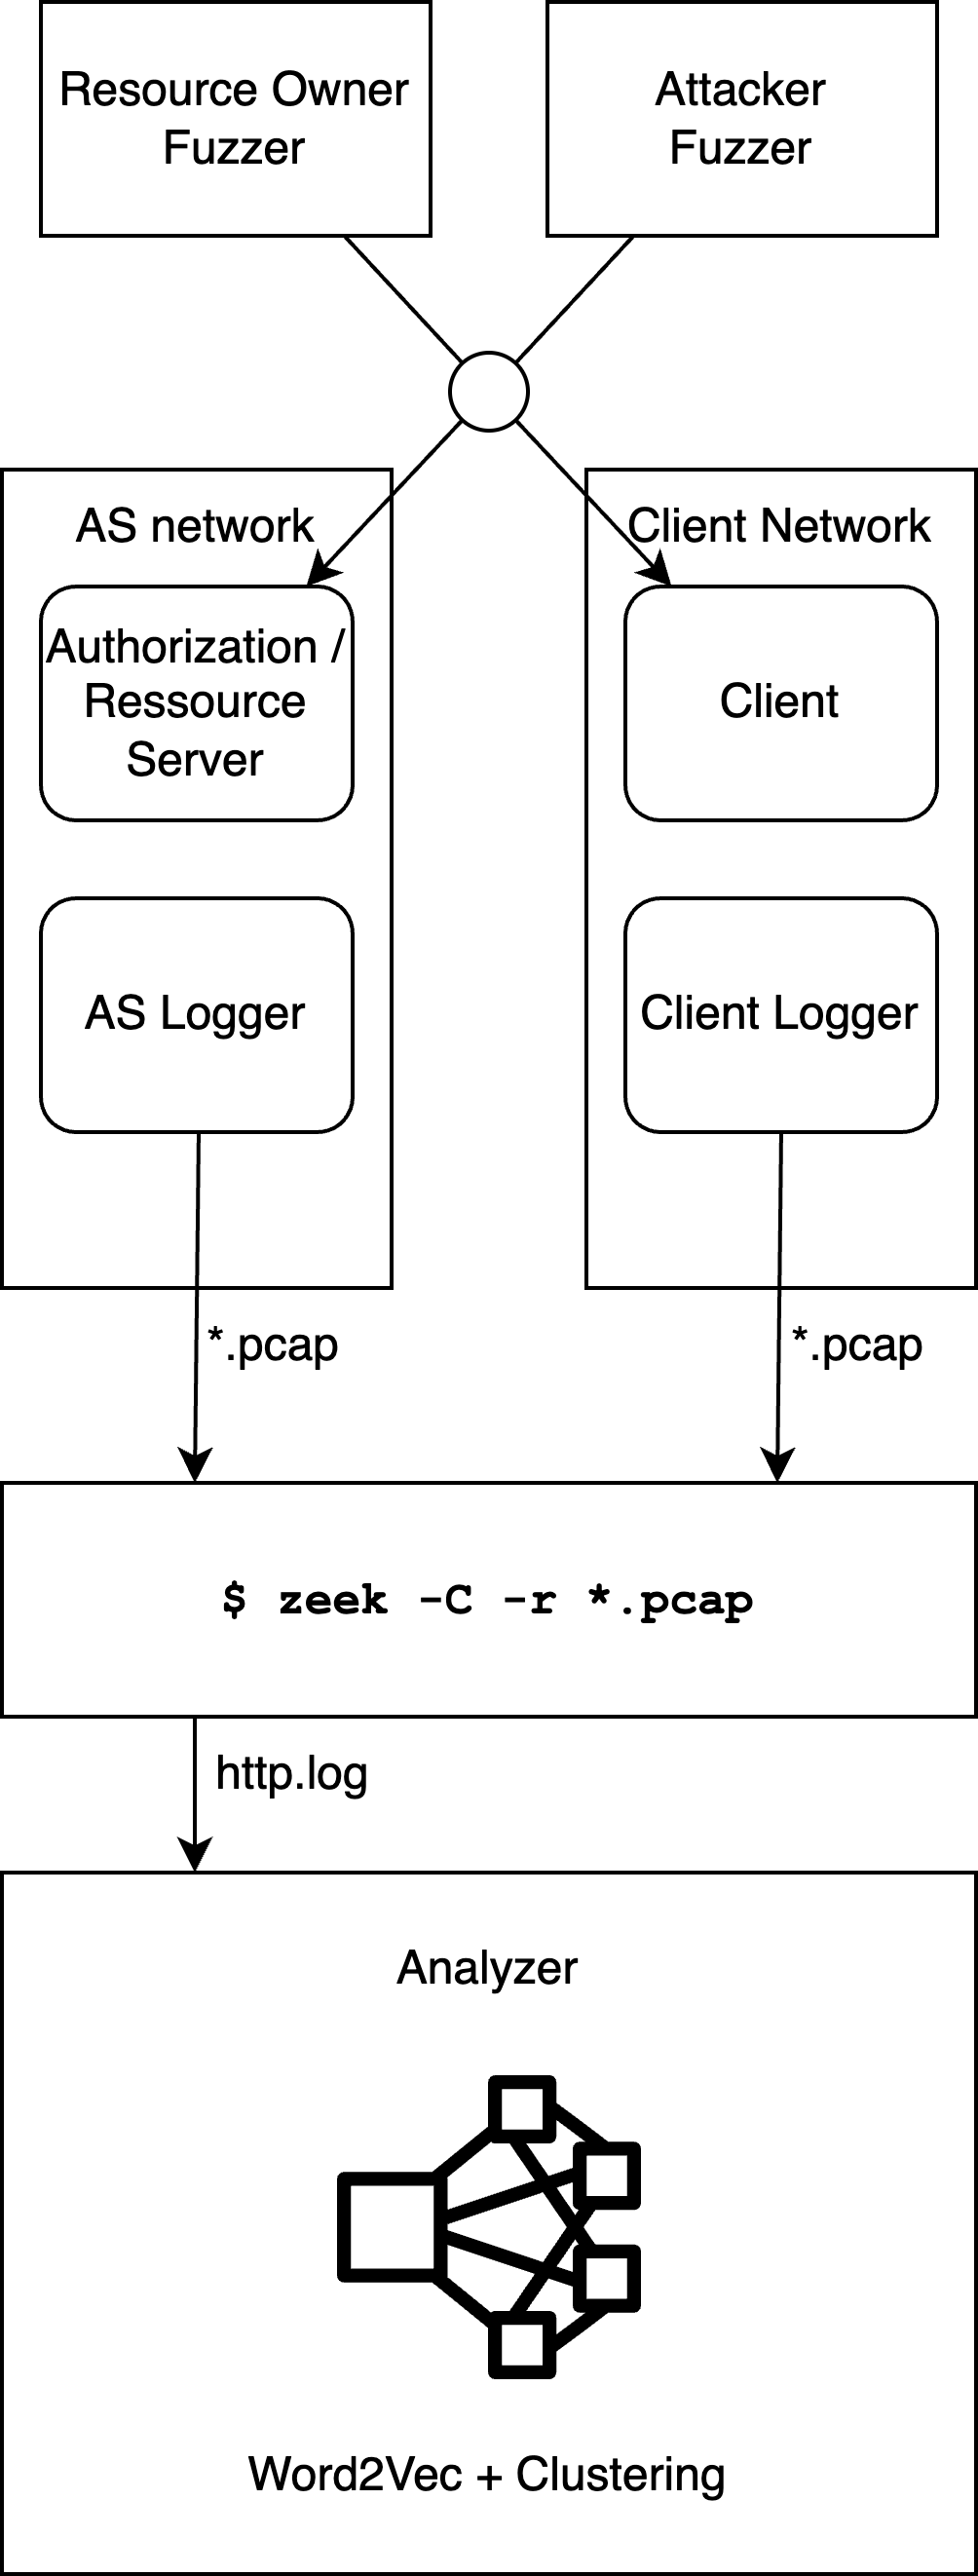
\includegraphics[width=0.5\textwidth]{pic/experimental_setup.png}
	\unitlength=0.75mm
	\special{em:linewidth 0.4pt}
	\linethickness{0.4pt}
	\caption{Overview of the environment for the experiments}
	\label{fig:experimental_setup}
\end{figure}
\todo{Change k-Means to clustering in graphic}

\subsection{OAuth setup}
For this first part, an OAuth environment was implemented, which consists of several subsystems that are needed to execute the OAuth protocol flow. It consists of two independent networks. The first network contains the authorization provider, resource server and a logging service, and the second network contains the OAuth client service and a logging service. The loggers produce .pcap-files of all activity in their network using \emph{tcpdump}. The OAuth authorization framework is practice-oriented. Therefore, the network logs are divided between the auth provider and the client, as in practice, mostly two different parties run these services. 

\subsubsection{Authorization Server and Resource Server}
The implementation of the authorization server and resource server is forked from the \emph{authlib} project version 1.2.1 \cite{authlib2023}. More specifically the ``Flask OAuth Providers'' component is utilized for the authorization and resource server. To make the authorization process more vulnerable the mandatory PKCE feature was deactivated. Having the possibility to make adjustments like this, was the reason for forking the project, instead of importing it as a library. The authorization server implementation of \emph{authlib} offers four OAuth grants out of the box, which are among the most essential grants, namely ``Implicit Grant'', ``Authorization Code Grant'', ``Client Credentials Grant'', and ``Password Grant''. It also implements extensions like the ``Refresh Token Grant'' and the ``PKCE''-extension. Besides the authorization capabilities, the authlib implementation also offers a protected resource in the form of an API, which is only accessible by authorized clients. The protected endpoint it offers returns the username of the currently authorized user.

\subsubsection{Client}
The client is a simple static webpage that handles the authorization code flow. It can be used to generate traffic manually, but its primary purpose is to handle redirections as part of the different flows. It is written in HTML, CSS, and Javascript to utilize the Fetch API and the Browser Storage API. An implementation of redirect handling is shown in figure \ref{lst:redirect_handler}. The client is checking if the code query parameter is present in the currently active URL (line 6) when the page loads. If it is present it extracts it and retrieves an access token from the authorization server.

\begin{lstlisting}[language={java}, caption={Example implementation of authorization code handling at the client}, label={lst:redirect_handler}]
// fetch access token on page load, if the code query param is present
window.onload = function() {
	const params = new URLSearchParams(window.location.search);
	const client_id = "<pre-configured client ID>"

	if (params.has("code")) {
		const form = new FormData();
		form.append('grant_type', 'authorization_code');
		form.append('scope', '<some scope>');
		form.append('code', params.get("code"));
		form.append('client_id', client_id);
		fetch('<token endpoint of authorization server>', {
			method: 'POST',
			body: form
		})
	}
}
\end{lstlisting}

\subsection{Network setup and logging}
All services are hosted using containers in a docker environment. Technically these services are part of the same network at the docker host they are run on, but the logging services build overlay networks on the services they are observing. As visualized in figure \ref{fig:experimental_setup} there exist two logging services, one for the authorization and resource server and one for the client network. When the experiment environment is active, the logging services stream all network events to a .pcap file, which is accessible on the docker host machine through a volume. All communication is executed without TLS to be able to analyze all packets. In a real-world scenario this would not be the case, but mechanisms like proxies, who are acting as man-in-the middle would be able to inspect the network traffic unencrypted in that case as well.

\begin{minipage}\linewidth
\begin{lstlisting}[language={bash}, caption={Logger process}, label={lst:logging_service}] 
$ ethtool -K eth0 rx off tx off tso off;tcpdump -i eth0 -w /log/"$filename_prefix"-log-$(date +"%Y%m%d_%H-%M-%S").pcap
\end{lstlisting}
\end{minipage}

\subsection{Attacks}
\label{subsec:attacks}
For the attacks on OAuth several pre-conditions were established to make the OAuth environment vulnerable. PKCE as mentioned earlier has been made optional. There is not any CSRF protection in place, utilizing the state parameter. This leads to the attacks being harder to detect as omitting these parameters as an attacker, will not make a difference anymore compared to the usual traffic. Another assumption is that an attacker is at all times able to circumvent any whitelist for redirect URIs. This is simulated by allowing the URI of the attacker server in the securely implemented whitelist of \emph{authlib}. In addition, it is assumed that an attacker, who crafts a malicious link can make the victim use the malicious link, through phishing or similar techniques. Another precondition is that the victim is logged in at all times and if it is not logged in it will immediately complete the login process. To facilitate the attacks an attacker callback server has been implemented as well. Also, every HTTP request involved in an attack, even the ones where the victim is visiting a maliciously crafted URL is labeled with a special header \emph{X-Is-Attack} with the name of the attack as its value.

\subsubsection{Attacker callback server}
The attacker callback server is a service implemented using the Python ``http.server'' library, which serves the purpose of a callback handler for attacks that redirect the victim's OAuth flows to the attacker. This means if an authorization code or access token ends up being redirected to this callback server it immediately completes OAuth flows with the stolen authorization codes or access tokens and generates traffic at the auth orization server like this. An example implementation for such a callback handler is shown in figure \ref{lst:attacker_server}. The ``do\_GET'' method (line 2) is executed, whenever a GET request reaches the attacker server. If this request contains an authorization code parameter (line 7), the server tries to redeem it at the authorization server (line 16). The server then tries to access protected data at the resource server (line 21).

\begin{minipage}\linewidth
\begin{lstlisting}[language={python}, caption={Example implementation of an attacker server, which handles redirections}, label={lst:attacker_server}] 
class OAuthCallback(BaseHTTPRequestHandler):
    def do_GET(self):
        parsed_url = urlparse(self.path)
        query_params = parse_qs(parsed_url.query)

		# Abort if there is no 'code' parameter present.
        assert query_params["code"] is not None

		# Fetch access token with code
        auth_code=query_params["code"]
        data = {"grant_type": "authorization_code",
                  "code": auth_code,
                  "redirect_uri": REDIRECT_URI,
                  "client_id": CLIENT_ID,
                  "client_secret": ""}
        res = r.post(f"{AUTHORIZATION_SERVER_URL}/oauth/token", data=data)
        access_token_data = res.json()

        # Utilize stolen access token
        headers = {"Authorization": f"Bearer {access_token_data['access_token']}"}
        res = r.get(f"{RESOURCE_SERVER_URL}/api/me", headers=headers)
        print("whoami:", res.content)
\end{lstlisting}
\end{minipage}

\subsubsection{Arbitrary redirect URI}
The first attack implemented is making the victim start an OAuth flow using the authorization code grant, but redirecting it to the attacker callback server after authorization. This is done by simply exchanging the value of \emph{redirect\_uri} parameter to the location of the attacker callback server. The callback server then uses the received authorization to redeem an access token at the authorization server as displayed and already explained in figure \ref{lst:attacker_server}. The attacker then uses the access token to fetch protected resources. This is a very basic attack and assumes that there is not any kind of whitelist in place like it is simulated in the experiment environment. However, there are more sophisticated versions of this attack utilizing the e.g. \emph{Evil Slash} \cite{wang2019make} trick mentioned in Section \ref{threat:T1}. 

\subsubsection{Arbitrary redirect URI using ``Evil Slash''}
The evil slash attack is based on the fact that the parsing of URLs of browsers might mismatch the way the parser for a whitelist parses a given URL. There are two examples given by the research of Wang et al. that are related to handling forward and backward slashes as path separators. Suppose either the whitelist parser or the browser URL parser treats some slash as a path separator while the other parser does not. In that case, this behaviour can be exploited to circumvent the whitelist of the authorization server. These two versions were implemented in the experiments by crafting a URL, which relies on this type of vulnerability.

\subsection{Network data generation}
The above-described services create a complete environment for executing valid OAuth flows and attacks on OAuth. To generate the data set for the analysis, a generator script was implemented in Python to utilize the whole setup to produce network logs. The approach for the generation is to mostly produce random valid traffic in the network. Meanwhile, at random some amount of attacks are executed as well, with a probability of 5\%, to simulate subtle attacks on the authorization. As the logging services are always listening, they produce network log files, which are then extracted after a reasonable amount of time.

\section{Implementation of analysis algorithms}
The last remaining part of the experimental setup is the intrusion detection mechanism. Based on the type of attacks implemented the decision was made, to analyze the logs produced by the authorization server, because the attack traffic appears in the network of this entity. The input for this part of the experiments is therefore the network log file produced by the logger of the authorization server overlay network. This file is passed to the data preprocessing step initiated by \emph{zeek}. The approach for the next step after the preprocessing, the detection step is based on previous studies \cite{carrasco2018unsupervised} \cite{zhuo2017network}, which had success in utilizing word2vec word embeddings to detect malicious network traffic even in small datasets. Therefore the same idea was chosen for this work to encode textual data, to enable clustering methods of the logs to reveal anomalies in the network data.

\subsection{Data preprocessing}
\label{subsec:dataset}
The first step of processing the data is to run it through the \emph{zeek IDS} to produce ``zeek-logs''. Zeek splits the data into different processed log files depending on the protocol of the packets. Since this research focuses on attacks on a specific protocol in the application layer, all logs, except for the http-log, get omitted. Another important detail is, that while producing the zeek-logs a ``zeek-script'' is loaded to preserve the HTTP headers in the HTTP log of zeek, as the headers include the labeling for the attacks and are not included by default in the zeek http-logs. The next steps of processing and the entire analysis from now on are executed using Python and popular data science libraries, which are mostly available for this programming language. Zeek supports the \emph{zat} library for Python, which allows for converting the zeek log into a data frame for the popular data-science library \emph{pandas}. After converting the zeek logs to a data frame a column gets added called ``is\_attack''. The column holds a flag for the row in the log if it is involved in an attack. The values for ``is\_attack'' get generated, by checking if the ``client\_header'' row includes a header called ``X-Is-Attack''. Afterwards, the ``X-Is-Attack''-header gets cleared from the header columns, as they are not a natural part of the traffic. The resulting matrix contains 34 columns, which carry different kinds of data like the URI of the request, the source and destination IPs, the HTTP method used, etc (compare Table \ref{tab:dataframe} for a full list of columns).


\begin{table}[]
	\caption{List of all features, which represent a column in the network data matrix after the first pre-processing step.}
	\label{tab:dataframe}
		\begin{tabular}{|l|l|l|}
		\hline
		\begin{tabular}[c]{@{}l@{}}uid\\ id.orig\_h\\ id.orig\_p\\ id.resp\_h\\ id.resp\_p\\ trans\_depth\\ method\\ host\\ uri\\ referrer\\ version\\ user\_agent\end{tabular} & \begin{tabular}[c]{@{}l@{}}origin\\ request\_body\_len\\ response\_body\_len\\ status\_code\\ status\_msg\\ info\_code\\ info\_msg\\ tags\\ username\\ password\\ proxied\end{tabular} & \begin{tabular}[c]{@{}l@{}}orig\_fuids\\ orig\_filenames\\ orig\_mime\_types\\ resp\_fuids\\ resp\_filenames\\ resp\_mime\_types\\ client\_header\_names\\ client\_header\_values\\ server\_header\_names\\ server\_header\_values\\ is\_attack\end{tabular} \\ \hline
		\end{tabular}
		\end{table}

\subsection{Encoding of URI data using word embeddings}
The attacks in this experiment (see Section \ref{subsec:attacks}) are based on tampering with the application layer data by manipulating the HTTP request-line and its query parameters. This data, therefore, is crucial for achieving the goal of detecting anomalies in the network logs. Hence, the previously prepared data frame columns, which hold the relevant data, are the \emph{uri} and the \emph{method} columns. Listing \ref{lst:tokenization} now shows the first necessary step for implementing the Word2Vec embeddings, the tokenization. Line two of the listing shows an important decision for the tokenization approach. The URI string is split into multiple parts by isolating every query parameter and separating every value from its query parameter key.

\begin{minipage}\linewidth
	\begin{lstlisting}[language={python}, caption={Tokenization of the features for word embeddings}, label={lst:tokenization}] 
		# Create token input list of all 'uri' and 'method' values for the word2vec model
		tokenized_uri = selected_features_df['uri'].apply(lambda x: re.split('[/?&=]', x))
		tokenized_method = selected_features_df['method'].apply(lambda x: [x])
		all_tokens = tokenized_method + tokenized_uri
	\end{lstlisting}
\end{minipage}


With the now acquired list of token combinations, a Word2Vec model is trained using the \emph{gensim.models} library \cite{gensim2021}. The model's hyperparameters get configured by setting the parameters of the constructor of the Word2Vec class. In this case, shown in Listing \ref{lst:word2vec} in line 1, the \emph{min\_count} variable is set to \emph{1} because, especially for anomaly detection, it makes sense to include one-time occurrences of words for the model's training, which would be omitted otherwise. The \emph{window\_size} defines what distance of words is still considered as the context of a given word. Finding the optimal value for this hyperparameter is the subject of the experiments and is discussed later in the results. The \emph{vector\_size} parameter determines the size of the dimension of the word embeddings produced by the model. Higher values produce more nuanced embeddings but also require more computational effort. Similar previously cited research by Zhou et al. \cite{zhuo2017network} uses a vector size of 300, which is why this number was chosen for the experiments of this work as well. The last parameter, the \emph{workers} parameter, describes the number of CPU cores to be involved in the training in parallel. With the previously generated tokens and the chosen hyperparameters, a Word2Vec model gets trained, and the embeddings are created and saved to a new column called \emph{embeddings} (see lines 4-9).


\begin{minipage}\linewidth
	\begin{lstlisting}[language={python}, caption={Creation of Word2Vec model and word embeddings}, label={lst:word2vec}] 
		# Create word2vec model
		word2vec_model = Word2Vec(all_tokens, vector_size=300, window=7, min_count=1, workers=4)
		
		# Utilize the Word2Vec model to apply embeddings to 'uri' and 'method' values
		selected_features_df['uri_embedding'] = tokenized_uri.apply(lambda x: sum(word2vec_model.wv[t] for t in x))
		selected_features_df['method_embedding'] = tokenized_method.apply(lambda x: sum(word2vec_model.wv[t] for t in x))
		
		# Combine embeddings into a single feature for clustering
		selected_features_df['embedding'] = selected_features_df.apply(lambda row: row['uri_embedding'] + row['method_embedding'], axis=1)
	\end{lstlisting}
\end{minipage}

\subsection{Clustering}
\todo{Write about the implementation of k-Means and Self-Organizing Maps}
Two clustering algorithms for anomaly detection are implemented to test the detection rate of attacks in the network logs based on previously generated word embeddings. The first algorithm is the \emph{k-Means clustering algorithm}, and the second is self-organizing maps. For classifying the clusters, a similarly simple approach to that used in the work of Nalavade et al. \cite{nalavade2014} is chosen by defining a threshold for the cluster size, after which a cluster is labeled as an attack cluster.

\subsubsection{k-Means}

\subsubsection{Self-organizing maps}

\section{Results}
This section describes the results of the intrusion detection approach conducted in this work on the self-generated dataset.

\begin{table}[H]
	\caption{Results of Intrusion Detection using Word2Vec and Clustering algorithms}
	\label{tab:results}
	\begin{tabular}{|l|l|l|}
	\hline
					   & \textbf{k-Means} & \textbf{Self-Organizing Maps} \\ \hline
	\textbf{Accuracy}  & 0.993            & 0.987                         \\ \hline
	\textbf{Yield}     & 1.0              & 1.0                           \\ \hline
	\textbf{Precision} & 0.637            & 0.463                         \\ \hline
	\end{tabular}
\end{table}

\subsection{Dataset generation}
The dataset, as described in Section \ref{subsec:dataset}, consists of records representing the generated HTTP network traffic over a fixed period of time. For this analysis, a dataset containing 3627 records is generated containing 44 records, which are requests involved in the attacks on the OAuth protocol. All implemented attacks are based on tampering with the query parameters of the requests to interfere with the OAuth redirection flow. As the goal of the analysis is to detect anomalies in the traffic, the dataset is generated in a way that at random around one percent of the generated traffic is attacker traffic. Table \ref{tab:record_attack} shows an example of an attack record, while Table \ref{tab:record_traffic} shows examples of non-attack records.

\begin{table}[H]
	\caption{Representation of a record of the dataset containing a request involved in an attack}
	\label{tab:record_attack}
	\begin{tabular}{|l|l|l|l|}
	\hline
	\textbf{method} & \textbf{uri}                                                                                                                                                    & \textbf{is\_attack} & \textbf{cluster} \\ \hline
	GET             & \begin{tabular}[c]{@{}l@{}}/oauth/authorize\\ ?response\_type=code\\ \&client\_id=A30qfzW7fbvhAN4OtIq4ZNFR\\ \&redirect\_uri=http://localhost:8081\end{tabular} & 1                   & 2                \\ \hline
	\end{tabular}
\end{table}


\begin{table}[H]
	\caption{Representation of records of the dataset containing requests involved in usual traffic}
	\label{tab:record_traffic}
	\begin{tabular}{|l|l|l|l|}
	\hline
	\textbf{method} & \textbf{uri}                                                                                                                                                                                           & \textbf{is\_attack} & \textbf{cluster} \\ \hline
	GET             & \begin{tabular}[c]{@{}l@{}}/?next=http://localhost:5123/oauth/authorize\\ ?response\_type=code\\ \&client\_id=A30qfzW7fbvhAN4OtIq4ZNFR\\ \&redirect\_uri=http://localhost:8080/index.html\end{tabular} & 0                   & 0                \\ \hline
	GET             & /                                                                                                                                                                                                      & 0                   & 0                \\ \hline
	POST            & /create\_client                                                                                                                                                                                        & 0                   & 0                \\ \hline
	\end{tabular}
\end{table}

\subsection{Word2Vec embeddings}
The Word2Vec embeddings for the textual data are the most crucial step for the detection, as the clustering algorithms work with the vectors produced by the word2vec algorithm. The vectors hold the knowledge about the relation of the individual pieces of the URIs and methods. Finding the best Word2Vec embeddings is achieved by tuning the window size hyperparameter. This parameter controls how many words around a word are considered related. In the case of the URI, this is the decision of whether, for example, a query parameter key should only relate to its direct value or if the combination of multiple query parameter key-value pairs is considered related. Experimenting with the window size hyperparameter shows that it does not affect the detection rate for both clustering algorithms in this environment of generated data. This circumstance could result from the short repetitive strings given to the algorithm as input. Even though there is randomization in the generated traffic for user IDs, Figure \ref{fig:word_embeddings3D} shows a very dense cluster for most of the non-attack traffic, meaning these embeddings have a close semantic meaning. Following along with the representation in Figure \ref{fig:word_embeddings3D} it stands out that there is a large cluster and some smaller outliers. The goal of the clustering algorithms in the next step is to capture this observation.

\begin{figure}[H]
	\sffamily\footnotesize
	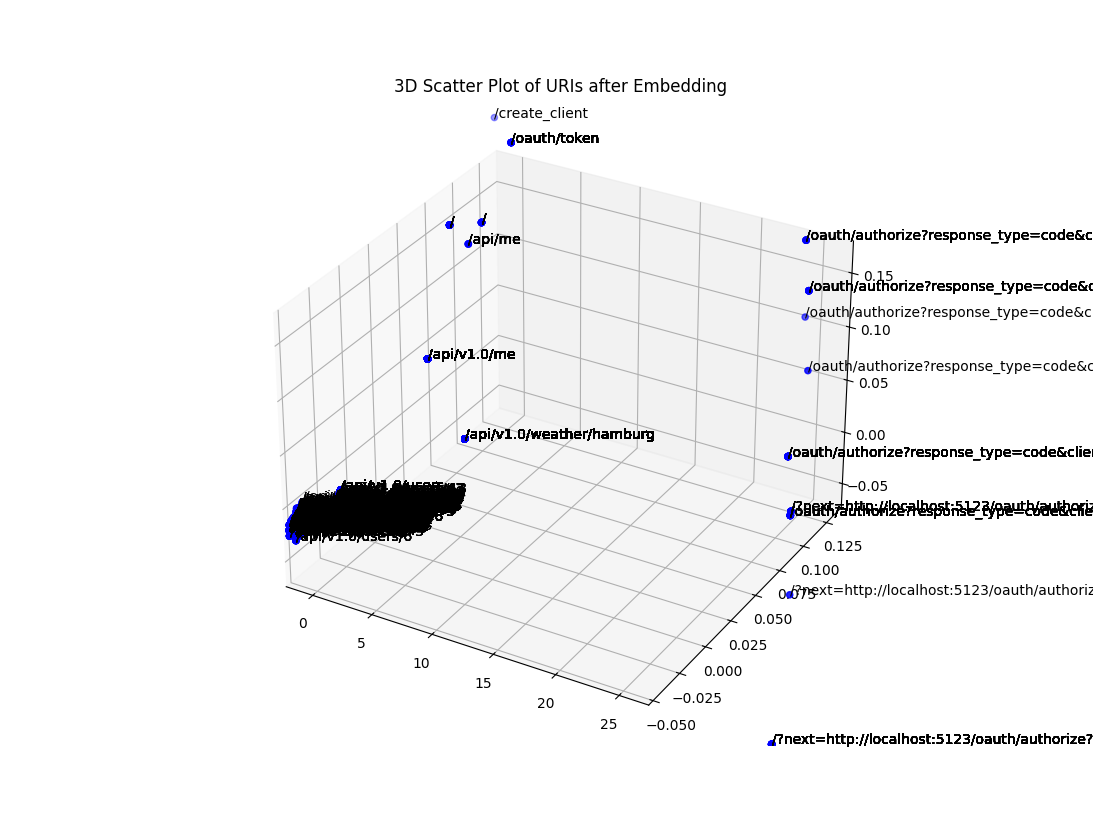
\includegraphics[width=1\textwidth]{pic/word_embeddings_3d.png}
	\unitlength=0.75mm
	\special{em:linewidth 0.4pt}
	\linethickness{0.4pt}
	\caption{Embedding Vectors normalized to 3 dimensions. Every vector is labeled with the corresponding URI, which led to its placement in the vector space}
	\label{fig:word_embeddings3D}
\end{figure}

\subsection{Clustering}
The last part of the detection chain aims to extract the anomalies to identify them as attacks. This goal is accomplished using unsupervised clustering algorithms described in Sections X and Y. 

\subsubsection{k-Means}
The k-means clustering results are influenced by how many clusters are chosen, as the algorithm works with a fixed amount of clusters from the beginning. Another circumstance to consider is the algorithm initializing its first cluster centroids randomly. This condition could influence the result. For this reason, a fixed seed for the randomizing of centroids was found to calculate the same clusters every time. A threshold for the cluster size compared to the total amount of records of 5\% was determined to identify the anomalies. Every cluster below this threshold is considered to include attacks. This calculation led to the results shown in Table \ref{tab:results}.

- Write about the results

- Write about what happens, when altering the cluster amount referencing Figure \ref{fig:kmeans_clusters_2} and Figure \ref{fig:kmeans_clusters_6}


\begin{figure}[H]
	\caption{Word2Vec and k-Means setting 2 clusters}
	\label{fig:kmeans_clusters_2}
	\sffamily\footnotesize
	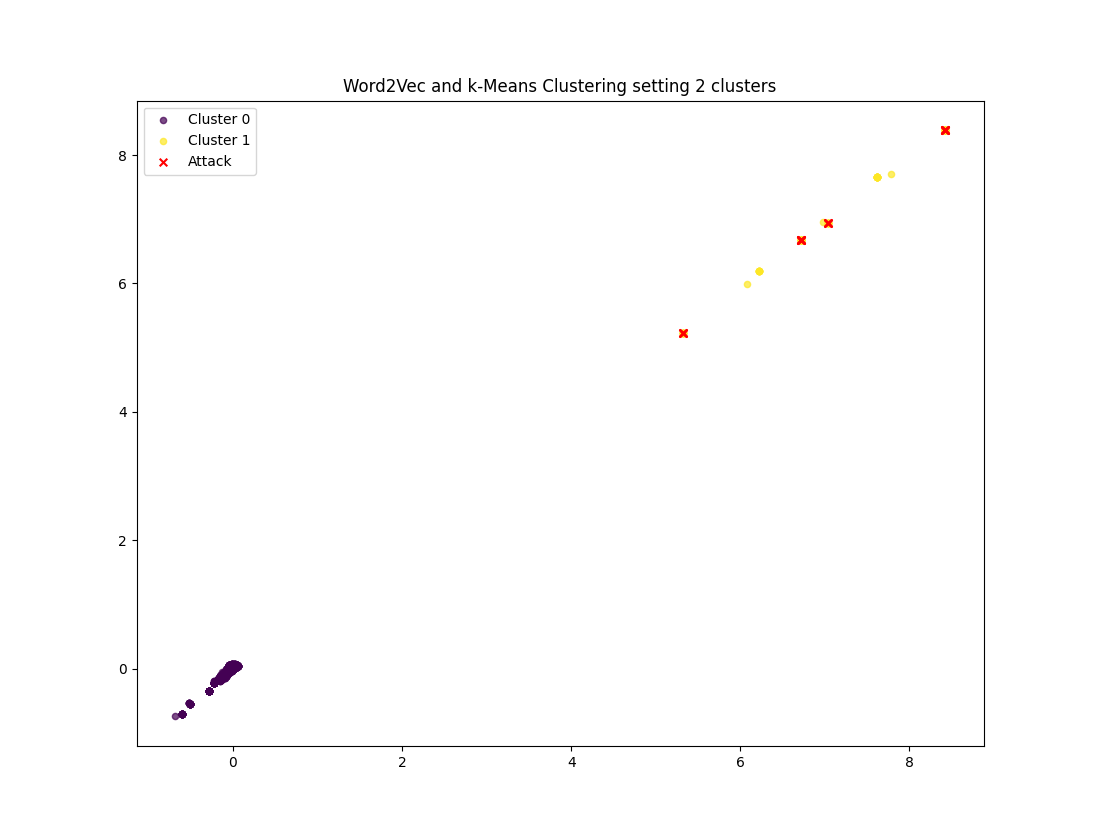
\includegraphics[width=1\textwidth]{pic/k_means_2.png}
	\unitlength=0.75mm
	\special{em:linewidth 0.4pt}
	\linethickness{0.4pt}
\end{figure}

\begin{figure}[H]
	\caption{Word2Vec and k-Means setting 6 clusters}
	\label{fig:kmeans_clusters_6}
	\sffamily\footnotesize
	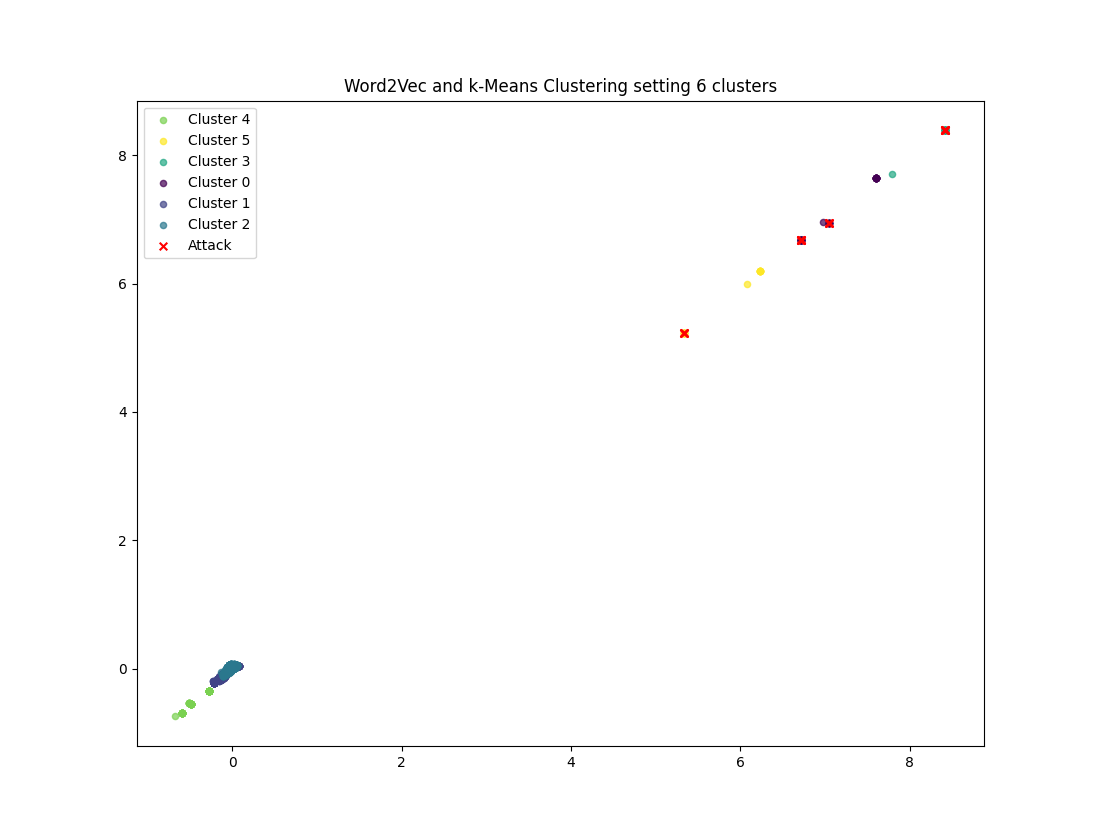
\includegraphics[width=1\textwidth]{pic/k_means_6.png}
	\unitlength=0.75mm
	\special{em:linewidth 0.4pt}
	\linethickness{0.4pt}
\end{figure}

\subsubsection{Self-Organizing Maps}
\begin{itemize}
	\item Write about hyperparameter tuning
	\item Write about Figure \ref{fig:som_clusters}
	\item Write about results Table \ref{tab:results}
\end{itemize}

\begin{figure}[H]
	\caption{Word2Vec and Self-Organizing Maps}
	\label{fig:som_clusters}
	\sffamily\footnotesize
	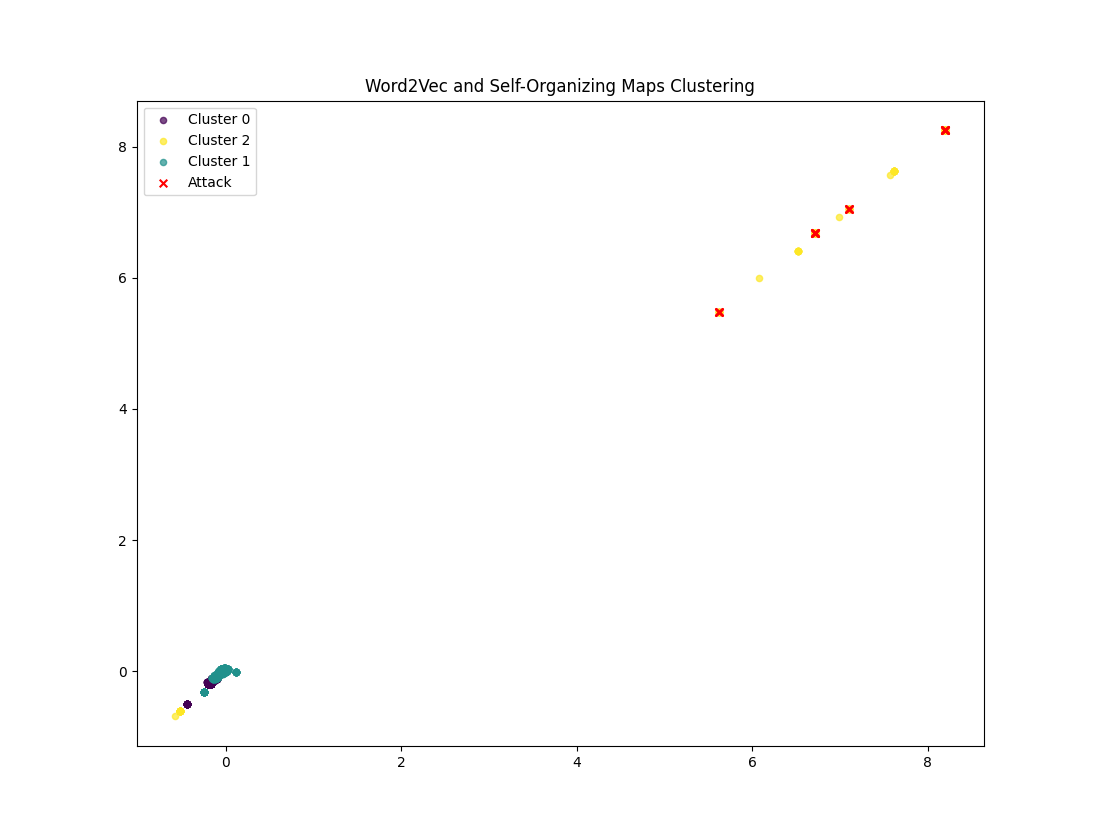
\includegraphics[width=1\textwidth]{pic/som_final.png}
	\unitlength=0.75mm
	\special{em:linewidth 0.4pt}
	\linethickness{0.4pt}
\end{figure}


\subsection{Discussion}

\begin{itemize}
	\item Discussion results
	\item (!) Discuss about data generation approach
	\begin{itemize}
		\item How realistic is the approach?
	\end{itemize}
	\item Discuss about relevance for real-world
\end{itemize}

\chapter{Conclusion}
\label{chap:conclusion}
\todo{Write Conclusion}



% =============================Literaturverzeichnis=============================
\begin{raggedright}         % Schaltet Blocksatz ab, erzeugt ein stimmigeres
                            %  Schriftbild im Literaturverzeichnis.
  \printbibliography        % Falls Biblatex verwendet wird.
  \label{sec:literaturverzeichnis}
\end{raggedright}


% ===================================Anhang=====================================
\appendix
\setcounter{figure}{0}
\renewcommand\thetable{A.\arabic{figure}}
\setcounter{table}{0}
\renewcommand\thetable{A.\arabic{table}}
\newpage
% ===

\chapter{Non encoded tables}

\begin{sidewaystable}
		\begin{xltabular}{\linewidth}{|l|l|l|l|l|l|l|l|l|l|l|l|l|l|l|l|l|X|}
		\hline
			~ & Mandatory PKCE & Random value state & Invalidation of access token & Invalidate state value & Simple String comparision & Avoid usage of grant types & Sender Constraint Access Token & Audience Constrained Access Token & Issuer identification & 303 Redirect & Not choosable client\_id & No redirect before authentication & No access token in uri & No third-party content on pages involved with OAuth & Appropriate Referer Policy & Open redirection countermeasures & Clickjacking countermeasures \\ \hline
			Insufficient Redirect URI Validation & ~ & ~ & ~ & ~ & x & ~ & ~ & ~ & ~ & ~ & ~ & ~ & ~ & ~ & ~ & x & ~ \\ \hline
			Credential Leakage via Referer Headers & x & ~ & x & x & ~ & x & ~ & ~ & ~ & ~ & ~ & ~ & ~ & x & x & ~ & ~ \\ \hline
			Credential Leakage via Browser History & ~ & ~ & x & ~ & ~ & x & ~ & ~ & ~ & ~ & ~ & ~ & x & ~ & ~ & ~ & ~ \\ \hline
			Mix-Up Attacks & ~ & ~ & ~ & ~ & ~ & ~ & ~ & ~ & x & ~ & ~ & ~ & ~ & ~ & ~ & ~ & ~ \\ \hline
			Authorization Code Injection & x & x & ~ & ~ & ~ & ~ & ~ & ~ & ~ & ~ & ~ & ~ & ~ & ~ & ~ & ~ & ~ \\ \hline
			Access Token Injection & ~ & ~ & ~ & ~ & ~ & x & ~ & ~ & ~ & ~ & ~ & ~ & ~ & ~ & ~ & ~ & ~ \\ \hline
			Cross-Site Request Forgery & x & x & ~ & ~ & ~ & ~ & ~ & ~ & ~ & ~ & ~ & ~ & ~ & ~ & ~ & ~ & ~ \\ \hline
			PKCE Downgrade Attack & x & ~ & ~ & ~ & ~ & ~ & ~ & ~ & ~ & ~ & ~ & ~ & ~ & ~ & ~ & ~ & ~ \\ \hline
			Access Token Leakage at the Resource Server & ~ & ~ & ~ & ~ & ~ & ~ & x & x & ~ & ~ & ~ & ~ & ~ & ~ & ~ & ~ & ~ \\ \hline
			307 Redirect & ~ & ~ & ~ & ~ & ~ & ~ & ~ & ~ & ~ & x & ~ & ~ & ~ & ~ & ~ & ~ & ~ \\ \hline
			Client Impersonating Resource Owner & ~ & ~ & ~ & ~ & ~ & ~ & ~ & ~ & ~ & ~ & x & ~ & ~ & ~ & ~ & ~ & ~ \\ \hline
			Authorization Server Redirecting to Phishing Site & ~ & ~ & ~ & ~ & ~ & ~ & ~ & ~ & ~ & ~ & ~ & x & ~ & ~ & ~ & ~ & ~ \\ \hline
			Unvalidated Redirects and Forwards & ~ & ~ & ~ & ~ & ~ & ~ & ~ & ~ & ~ & ~ & ~ & ~ & ~ & ~ & ~ & x & ~ \\ \hline
			Clickjacking & ~ & ~ & ~ & ~ & ~ & ~ & ~ & ~ & ~ & ~ & ~ & ~ & ~ & ~ & ~ & ~ & x \\ \hline
		\end{xltabular}
\end{sidewaystable}
\todo{Fix sideways table}
		
% ===========================Selbstständigkeitserklärung======================
\chapter*{Eidesstattliche Versicherung} % war: Selbständigkeitserklärung
\vspace{1cm}

\todo[noline]{Bitte verwenden Sie hier in jedem Fall die offizielle von der Prüfungsbehörde vorgegebene Formulierung der Selbständigkeitserklärung.}
%
Hiermit versichere ich an Eides statt, dass ich die vorliegende Arbeit
selbstständig verfasst und keine anderen als die angegebenen Hilfsmittel –
insbesondere keine im Quellenverzeichnis nicht benannten Internet-Quellen –
benutzt habe. Alle Stellen, die wörtlich oder sinngemäß aus Veröffentlichungen
entnommen wurden, sind als solche kenntlich gemacht. Ich versichere weiterhin,
dass ich die Arbeit vorher nicht in einem anderen Prüfungsverfahren eingereicht
habe und die eingereichte schriftliche Fassung der auf dem elektronischen
Speichermedium entspricht.

Ggf. streichen: Ich bin damit einverstanden, dass meine Abschlussarbeit in den
Bestand der Fachbereichsbibliothek eingestellt wird.

\makeatletter
Hamburg, den {\@date}
\makeatother

\vspace{2cm}
\rule{6cm}{0.25pt}\\
\makeatletter
{\@author} \par
\makeatother




% ================================Literaturliste-Muster==============================
\newpage
\thispagestyle{empty}
\label{sec:literaturliste}
\par\textbf{\textsf{Thema:}} Privacy Enhancing Technologies zum Schutz von Kommunikationsbeziehungen
\par\textbf{\textsf{Bearbeiter:}} Eva Musterfrau, Heinz Mustermann
\par\textbf{\textsf{Datum:}} \today
\bigskip
% ====> Delete me
\begin{tikzpicture}[overlay]
    \node[draw, blue, font=\sffamily\Large, xshift=70mm, yshift=0mm, rounded corners=1mm]{Muster der Literaturliste};
\end{tikzpicture}
% <==== /Delete me
\par\textbf{\Large\textsf{Literaturliste}}

% ================================Todo list==============================
\listoftodos
% \todototoc

\end{document}
